\documentclass{book}

\usepackage{ctex} % 排版中文文章
\usepackage{physics}
\usepackage{booktabs,tabularx,multicol,multirow} % 制作表格
\usepackage{appendix}
\usepackage{amsmath,amsthm,amssymb,amsfonts}    % 数学符号与字体

\usepackage{float}

\usepackage{hyperref}   % 添加超链接
\hypersetup{hidelinks}  % 把超链接周围的红框隐藏起来
% 设置超链接的样式
\hypersetup{
  colorlinks,    % 启用彩色链接
  % linkcolor=blue, % 定义链接的颜色为蓝色
  citecolor=blue, % 定义引用的颜色为蓝色
  % filecolor=blue, % 定义文件链接的颜色为蓝色
  % urlcolor=blue   % 定义URL链接的颜色为蓝色
}

\usepackage[dvipsnames]{xcolor} % 在latex中使用颜色

\usepackage{subfig,graphicx}    % 插入照片
\usepackage{enumitem}
\usepackage{lipsum,zhlipsum} %生成一些测试文本

\usepackage[left=2.0cm, right=2.0cm, top=2.5cm, bottom=2.5cm]{geometry} % 调整页边距
\usepackage{soul} % 高亮文本

% 字符编码和数学宏包
%\usepackage[utf8]{inputenc}
\usepackage{amsmath, amsthm, amsfonts, amssymb}
\usepackage{tikz} %很强大的绘图宏包

%自定义设置字体
\usepackage{fontenc}
\setmainfont{Times New Roman} % 设置英文衬线字体
%\setsansfont{Arial} % 设置英文无衬线字体
%\setmonofont{Courier New} % 设置英文等宽字体

% 表格宏包
\usepackage{multirow, booktabs} %两种不同处理表格,取决于不同情况的处理

% 页面和排版宏包
\usepackage{fullpage} %
\usepackage{enumitem} %处理列表(包括有序、无序两类)
\usepackage{fancyhdr} %
\usepackage{fontawesome}
\usepackage{geometry} %设置页面边距

% ============== 设置一个好看的页眉页脚款式 ===============
\geometry{ % 设置页面布局
  includeheadfoot, % 将页眉和页脚计算在页面范围内
  left=1in, % 设置左边距
  right=1in, % 设置右边距
  top=1in, % 设置上边距
  bottom=1in, % 设置下边距
}


% 其他页面设置
\geometry{margin=1in, headsep=0.75in}
% ====================================================

% 数学字体宏包
\usepackage{mathrsfs} %比如\mathcal,\mathscr等


% 图片和文本宏包
\usepackage{wrapfig} %处理浮动图片
\usepackage{graphicx}
\usepackage{caption}
\usepackage{setspace,calc} %前者设置距离,后者设置文本长度
\usepackage{multicol} %分列处理文本

% 公式宏包
\usepackage{cancel} %引入划去线
\usepackage[retainorgcmds]{IEEEtrantools} %表达式排版,比如align等 
\usepackage{empheq} %创建带有框和标签的数学公式

% 框架和颜色宏包
\usepackage{framed} %边框
\usepackage[most]{tcolorbox}
\colorlet{shadecolor}{orange!15} %颜色自定义

% ======= 定理环境边框 ======
\definecolor{browna}{rgb}{0.76,0.72,0.65}
\definecolor{brownb}{rgb}{0.71,0.69,0.65}
\definecolor{blacka}{RGB}{245,245,245}





%%%%%%%%%%%%%%%%%%%
\newtheorem{remark}{Remark}
\newtheorem{example}{Example}

% \newtcbtheorem[number within=section]{example}{Example}{colback=OliveGreen!10,colframe=Green!70,fonttitle=\bfseries}{example}






\newtcbtheorem[number within=subsection]{theorem}{Theorem}{
  enhanced,
  sharp corners,
  attach boxed title to top left={
      yshifttext=-1mm
    },
  colback=white,
  colframe=brownb,
  fonttitle={\bfseries},
  fontupper={\kaishu\itshape},
  boxed title style={
      sharp corners,
      size=small,
      colback=brownb,
      colframe=brownb,
    },
  breakable  % 添加这一行以启用自动断页
}{thm}


\newtcbtheorem[number within=subsection]{lem}{Lemma}{
  enhanced,
  sharp corners,
  attach boxed title to top left={
      yshifttext=-1mm
    },
  colback=white,
  colframe=brownb,
  fonttitle=\bfseries,
  boxed title style={
      sharp corners,
      size=small,
      colback=brownb,
      colframe=brownb,
    },
  breakable  % 添加这一行以启用自动断页 
}{lem}

\newtcbtheorem[number within=subsection]{cor}{Corollary}{
  enhanced,
  sharp corners,
  attach boxed title to top left={
      yshifttext=-1mm
    },
  colback=white,
  colframe=brownb,
  fonttitle=\bfseries,
  boxed title style={
      sharp corners,
      size=small,
      colback=brownb,
      colframe=brownb,
    },
  breakable  % 添加这一行以启用自动断页 
}{cor}

%---------------优雅的插入MATLAB代码---------%
\usepackage{lipsum,zhlipsum} %生成一些测试文本
\usepackage{listings,matlab-prettifier} % MATLAB 美化包
\lstset{
  style=Matlab-editor,
  numbers      = left,
  frame        = single,
}

\newtcbtheorem[number within=subsection]{definition}{Definition}{
  enhanced,
  sharp corners,
  attach boxed title to top left={
      yshifttext=-1mm
    },
  colback=white,
  colframe=browna,
  fonttitle=\bfseries,
  boxed title style={
      sharp corners,
      size=small,
      colback=browna,
      colframe=browna,
    },
  breakable  % 添加这一行以启用自动断页 
}{defn}






% ========= 标题、作者配置 =====


\usepackage{titling} % 自定义标题


% ============================

\usepackage{hyperref}
\title{RKDG Primer}
\author{张阳}
\date{\today}
\begin{document}
\maketitle
\tableofcontents
\newpage
\chapter{快速实现}
\section{引言}
\begin{figure}[ht]%
    \centering
    \subfloat[$t=0s$]{
        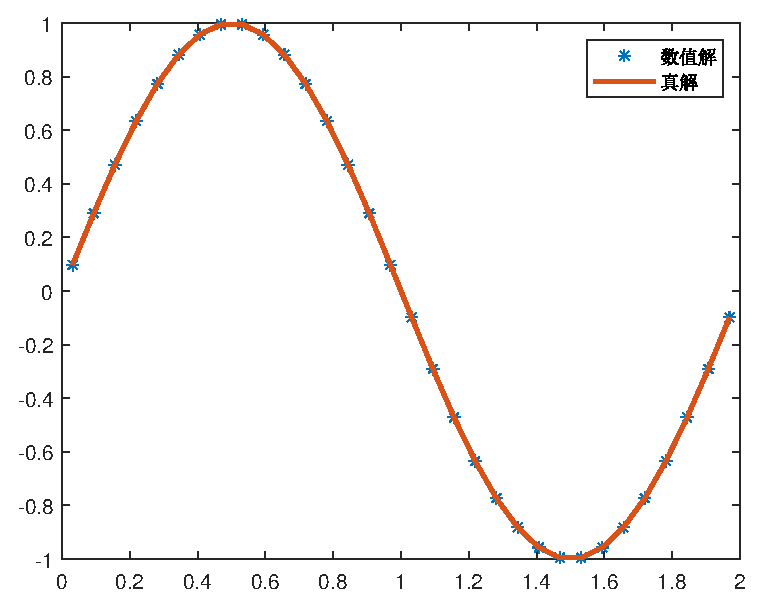
\includegraphics[width=0.3\linewidth]{fig/example1-t=0.0.eps}
    }\quad
    \subfloat[$t=0.2s$]{
        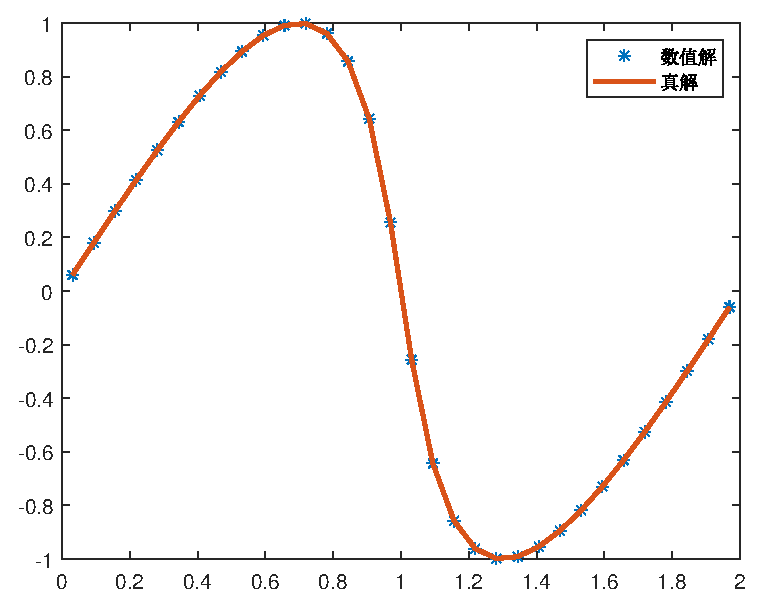
\includegraphics[width=0.3\linewidth]{fig/example1-t=0.2.eps}
    }\\
    \subfloat[$t=0.4s$]{
        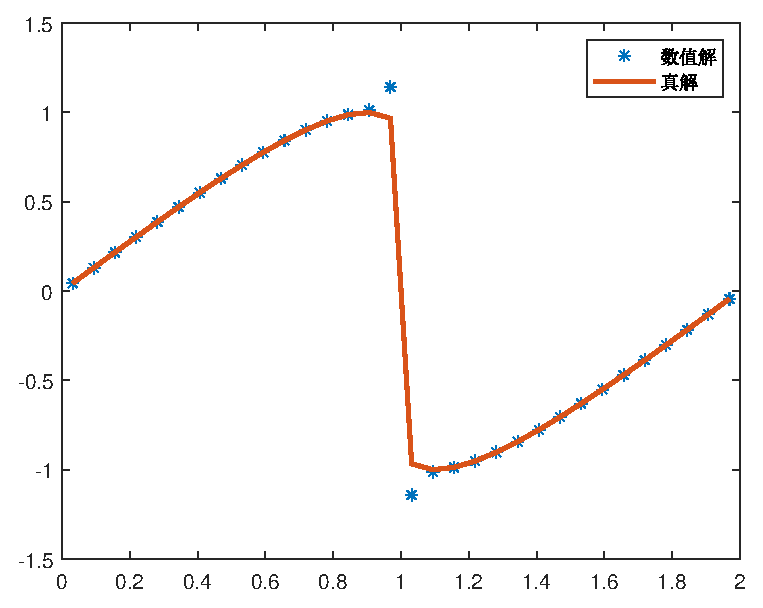
\includegraphics[width=0.3\linewidth]{fig/example1-t=0.4.eps}
    }\quad
    \subfloat[$t=0.6s$]{
        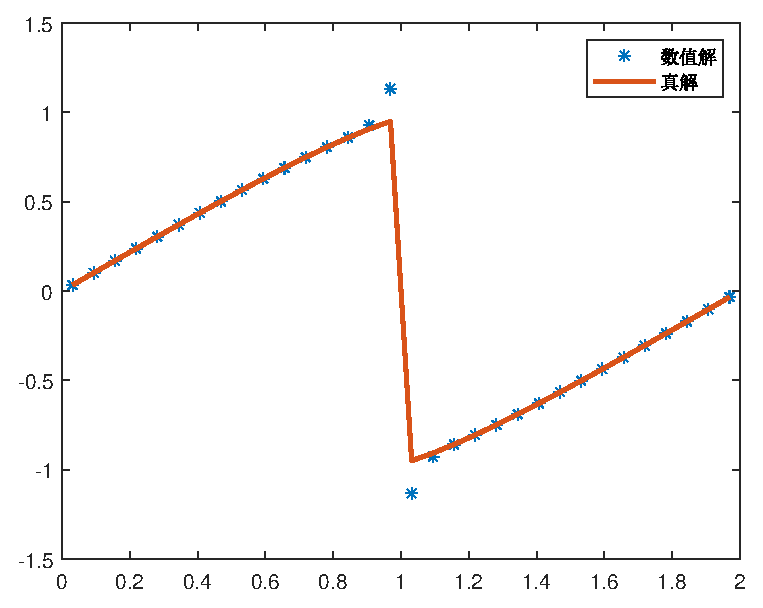
\includegraphics[width=0.3\linewidth]{fig/example1-t=0.6.eps}
    }\\
    \caption{上图为burgers方程在初值条件为$u=\sin(x)$时的演变}
    \label{间断示例}
\end{figure}


本文使用的数值方法为间断有限元discontinuous Galerkin (DG)法.让我们先简要回顾一下DG方法的历史.1973年,Reed和Hill\cite{Reed_Hill}在中子传输框架下提出了第一个不连续Galerkin(DG)方法.然后,Cockburn等人在一系列论文中 \cite{RKDG2,RKDG3,RKDG4,RKDG5} 对DG方法进行了重大发展,其中他们建立了一个框架,使用显式、非线性稳定的高阶Runge-Kutta时间离散化和DG空间离散化,使用精确或近似的Riemann解算器作为界面通量和总变差有界(TVB)限制器\cite{TVB},以实现对强不连续性的本质非振荡性.从那时起,这些方案被称为RKDG方法.但是,即使初始条件足够平滑,解决\eqref{equ:双曲守恒}也不容易,因为解可能包含强不连续性.不连续Galerkin(DG)方法可以捕捉弱不连续性而无需进一步修改.然而,对于存在强不连续性的问题,数值解可能在强震荡或接触不连续性附近具有显著的虚假震荡,特别是对于高阶数值方法而言.控制这些虚假震荡的常见策略是应用非线性限制器.

通常,使用限制器的过程可以分为两个步骤.首先,需要确定“坏单元”(也称为“有问题的单元”),即包含间断的单元,这些单元需要进行限制.其次,需要在这些“坏单元”中修正DG多项式解.由于守恒的要求,需要保证单元平均值不变,并且减小振荡.

在第一部分中,我们通常使用“坏单元”或称为间断指示器,这些指示器包括基于最小模型的指示器\cite{RKDG2}、基于力矩的指示器\cite{基于力矩的指示器}、改进的力矩指示器\cite{改进的基于矩的限制器}、以及基于DG超收敛性质的KXRCF指示器\cite{基于DG超收敛性质的KXRCF指示器}.

在第二部分中,一种限制器属于斜率型限制器,例如minmod类型限制器\cite{RKDG2,RKDG3,RKDG4,RKDG5},基于矩的限制器\cite{基于矩的限制器}和改进的基于矩的限制器\cite{改进的基于矩的限制器}等.它们的优点是可以在强间断附近有效抑制伪振荡的出现,但付出的代价是在解的光滑极值点处有可能降低格式的数值精度.另一种限制器基于加权本质非振荡(WENO)方法\cite{WENO1,WENO2,WENO3,WENO4,WENO5},它可以在平滑区域中实现高阶精度,并在强不连续性附近保持本质非振荡性质.WENO 格式一经提出,便引起人们的广泛关注,近二十年来,WENO 的各种变形格式层出不穷.例如:经典的WENO限制器(WENO-js)\cite{WENO-js1,WENO-js2},Hermite WENO限制器(HWENO)\cite{HWENO1,HWENO2},中心型 WENO 限制器(CWENO)\cite{CWENO},WENO-M限制器\cite{WENO-M},WENO-Z限制器\cite{WENO-Z}.但另一方面,基于WENO的限制器需要更广泛的空间模板来获得高阶方案.因此,在多维问题中,特别是在非结构化网格上,如三角形网格或四面体网格中实现它们是困难的.

\section{符号说明}
$\hat{h}$ 数值通量

\begin{equation}
    \Delta_{+} w_{j}=w_{j+1}-w_{j}, \quad \Delta_{-} w_{j}=w_{j}-w_{j-1}
\end{equation}

\section{一维标量}
离散格式推导与稳定性证明见\cite{RN16}
\subsection{控制方程}
\begin{equation}
    u_t+f(u)_x = 0
\end{equation}
\subsection{空间离散格式}

$x_{l}=x_{\frac{1}{2}}<x_{\frac{3}{2}}<\cdots<x_{N-\frac{1}{2}}<x_{N+\frac{1}{2}}=x_{r} .$

We define cells, cell centers, and cell sizes by

$\begin{array}{l}
        I_{i} \equiv\left[x_{i-\frac{1}{2}}, x_{i+\frac{1}{2}}\right], \quad x_{i} \equiv \frac{1}{2}\left(x_{i-\frac{1}{2}}+x_{i+\frac{1}{2}}\right) \\
        \Delta x_{i}=x_{i+\frac{1}{2}}-x_{i-\frac{1}{2}}, \quad i=1,2, \cdots, N .
    \end{array}$

\begin{equation}
    u_{h}(x, t)=\sum_{l=0}^{k} u_{i}^{(l)}(t) v_{l}^{(i)}(x), \quad x \in I_{i}
\end{equation}
其中 $u_i^{(l)}(t)$ 为自由度(degrees of freedom:dof)或矩,$v_l^{(i)}(x)$ 为基函数.当基函数为正交函数时,$u_i{(l)}(t)$ 的定义为:
\begin{equation}
    u_{i}^{(l)}(t)=\frac{1}{a_{l}} \int_{I_{i}} u_{h}(x, t) v_{l}^{(i)}(x) d x \quad l=0,1, \ldots, k
\end{equation}
其中 $a_{l}=\int_{I_{i}}\left(v_{l}^{(i)}(x)\right)^{2} d x$
\begin{remark}
    如果基函数不是正交函数,需要先求出质量矩阵的值,再求其逆矩阵.
\end{remark}
\begin{remark}
    当基函数为正交函数时,第一个自由度的值,即为函数在小区间上的积分平均值.
\end{remark}
\begin{equation}
    \left\|v_{l}^{(j)}(x)\right\|^{2} \dfrac{\dd}{\dd t} u(t)+\left[\Delta_{-}\left(v_{l}^{(j)}\left(x_{j+1 / 2}\right) f_{j+1 / 2}\right)\right]-\int_{I_{j}} f\left(u^{h}(x, t)\right) \dfrac{\dd}{\dd x} v(x) \dd x=0
\end{equation}

这里推导的时候要用到xx,算一下看看
\begin{equation}
    \frac{\dd}{\dd t}u+\frac{\dd}{\dd x}f=0
\end{equation}

\subsection{实例}
\begin{example}
    光滑问题:
    \begin{equation}
        u_t+u_x=0,u(x,0)=\sin x,0\leqslant x\leqslant 2\pi
    \end{equation}
    周期边界条件

    解析解为:

    \begin{equation}
        u(x,t) = \sin(x-t)
    \end{equation}
\end{example}

\begin{example}
    % https://zhuanlan.zhihu.com/p/502638295
    间断问题:

    \begin{equation}
        u_{t}+\left(\frac{u^{2}}{2}\right)_{x}=0
    \end{equation}

    初值为:

    $u_0(x)=\sin(x)$

    计算域为 $[0,2\pi]$.

    $x=\pi$ 的地方会出现激波,激波出现的时间为 $t=1$.

    解析解使用特征线法求解.
\end{example}




\section{一维向量}

\begin{equation}
    \mathbf{U}_{t}+\mathbf{F}(\mathbf{U})_{x}=\mathbf{0}
\end{equation}

数值通量为:

\begin{example}
    \begin{equation}
        \begin{aligned}
            \rho(x, 0) & =1+0.2 \sin \pi x \\
            u(x, 0)    & =0.7              \\
            p(x, 0)    & =1
        \end{aligned}
    \end{equation}
    计算区域为 $[0,2]$, 周期边界条件,解析解为:
    \begin{equation}
        \begin{aligned}
            \rho(x, t) & =1+0.2 \sin \pi(x-0.7 t) \\
            u(x, t)    & =0.7                     \\
            p(x, t)    & =1
        \end{aligned}
    \end{equation}


\end{example}

\begin{example}
    Lax 激波管问题(shock–tube problem)\cite{RN109}:
    \begin{equation}
        \begin{aligned}
            (\rho, v, p) & =(0.445,0.698,3.528) & \text { 当 } x \leqslant 0 \text {, } \\
            (\rho, v, p) & =(0.5,0,0.571) \quad & \text { 当 } \quad x>0 \text {. }     \\
        \end{aligned}
    \end{equation}
    计算区域为 $[-5,5]$ 两瑞均是常数边界条件, 我们求解该问题至 $T=1.3$.
    \begin{figure}[htp]
        \centering
        \label{fig:}
        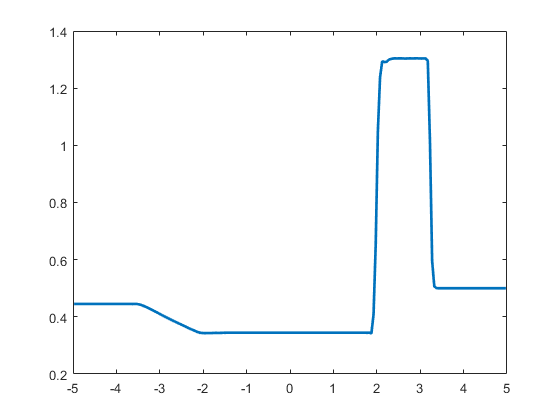
\includegraphics[width=0.7\linewidth]{fig/lax_problem.png}
        \caption{$M=50$,$N=200$,$P_2$,WENO-JS}
    \end{figure}

\end{example}
\section{二维标量}
% https://zhuanlan.zhihu.com/p/441631704

\section{二维向量}
\subsection{控制方程}
\begin{equation}
    \partial_{t} \boldsymbol{u}+\operatorname{div} \boldsymbol{f} (\boldsymbol{u})=0
\end{equation}
\subsection{空间离散格式}
在每个小区间上做二维积分:
\begin{equation}
    \frac{d}{d t} \int_{K} u_{h}(t, x) v_{h}(x) d x+\int_{K} \operatorname{div} \mathbf{f}\left(u_{h}(t, x)\right) v_{h}(x) d x=0, \forall v_{h} \in V_{h}
\end{equation}
\begin{equation}
    \dfrac{\dd}{\dd t} \int_{K} u(x, t) v(x) \dd x+\sum_{e \in \partial K} \int_{e} \mathbf{f}(u(x, t)) \cdot n_{e, K} v(x) \dd \Gamma-\int_{K} \mathbf{f}(u(x, t)) \cdot \operatorname{grad} v(x) \dd x=0
\end{equation}
\begin{remark}
    特别的,对于矩形网格,有:
\end{remark}
其中 $n_{e,K}$ 是边界 $e$ 的标准外法向量.由于函数在小区间边界上间断 $f(u)$ 在 $e$ 上没有定义,和一维的情况类似,需要使用数值通量$h_{e, K}\left(u_{h}\left(t, x^{\operatorname{int}(K)}\right), u_{h}\left(t, x^{\operatorname{ext}(K)}\right)\right)$代替$\mathbf{f}\left(u_{h}(t, x)\right) \cdot \mathbf{n}_{e, K}$, 其中:
\begin{equation}
    \begin{array}{l}
        u_{h}\left(t, x^{i n t(K)}\right)= \lim _{\substack{y \rightarrow x \\
        y \in K}} u_{h}(t, y),                                              \\
        u_{h}\left(t, x^{e x t(K)}\right)=\left\{\begin{array}{ll}
                                                     \gamma_{h}(x, t),           & \text { if } x \in \partial \Omega, \\
                                                     \lim _{\substack{y \rightarrow x                                  \\
                                                     y \in(K)^{c}}} u_{h}(t, y), & \text { otherwise. }
                                                 \end{array}\right.
    \end{array}
\end{equation}

% \begin{equation}
%     \int_{e} \mathbf{f}(u(x, t)) \cdot n_{e, K} v_{h}(x) d \Gamma \approx \sum_{l=1}^{L} \omega_{l} \mathbf{f}\left(u\left(x_{e l}, t\right)\right) \cdot n_{e, K} v\left(x_{e l}\right)|e|,
% \end{equation}
% \begin{equation}
%     \int_{K} \mathbf{f}(u(x, t)) \cdot \operatorname{grad} v(x) d x \approx \sum_{j=1}^{M} \underline{\omega}_{j} \mathbf{f}\left(u\left(x_{K j}, t\right)\right) \cdot \operatorname{grad} v\left(x_{K j}\right)|K| .
% \end{equation}

\begin{equation}
    h_{e, K}(a, b)=\frac{1}{2}\left[\mathbf{f}(a) \cdot n_{e, K}+\mathbf{f}(b) \cdot n_{e, K}-\alpha_{e, K}(b-a)\right] .
\end{equation}

\begin{example}
    光滑问题:初值为:
    \begin{equation}
        \begin{aligned}
            \rho(x,y,0) & = 1+0.2\sin(\pi(x+y)) \\
            u(x,y,0)    & = 0.7                 \\
            v(x,y,0)    & = 0.3                 \\
            p(x,y,0)    & = 1                   \\
        \end{aligned}
    \end{equation}
    周期边界条件

    准确解为:
    \begin{equation}
        \rho(x,y,t) = 1+0.2\sin(\pi(x+y-(u+v)t)),u=0.7,v=0.3,p=1
    \end{equation}
\end{example}



\begin{example}黎曼问题:
    % https://www.researchgate.net/publication/370612578_A_dissipation-dispersion_coupled_inequality_for_a_class_of_upwind_multi-resolution_WENO_schemes
    算例可参考:\cite{RN114}
    \begin{equation}
        (\rho, u, v, p)=\begin{cases}
            (0.138,1.206,1.206,0.029), & (x, y) \in[0,0.8) \times[0,0.8) \\
            (0.5323,1.206,0,0.3),      & (x, y) \in[0,0.8) \times[0.8,1] \\
            (0.5323,0,1.206,0.3),      & (x, y) \in[0.8,1] \times[0,0.8) \\
            (1.5,0,0,1.5),             & (x, y) \in[0.8,1] \times[0.8,1]
        \end{cases}
    \end{equation}
    $t_{end}=0.8$,网格为$400\times400$.

    \begin{figure}[ht]%
        \centering
        \subfloat{
            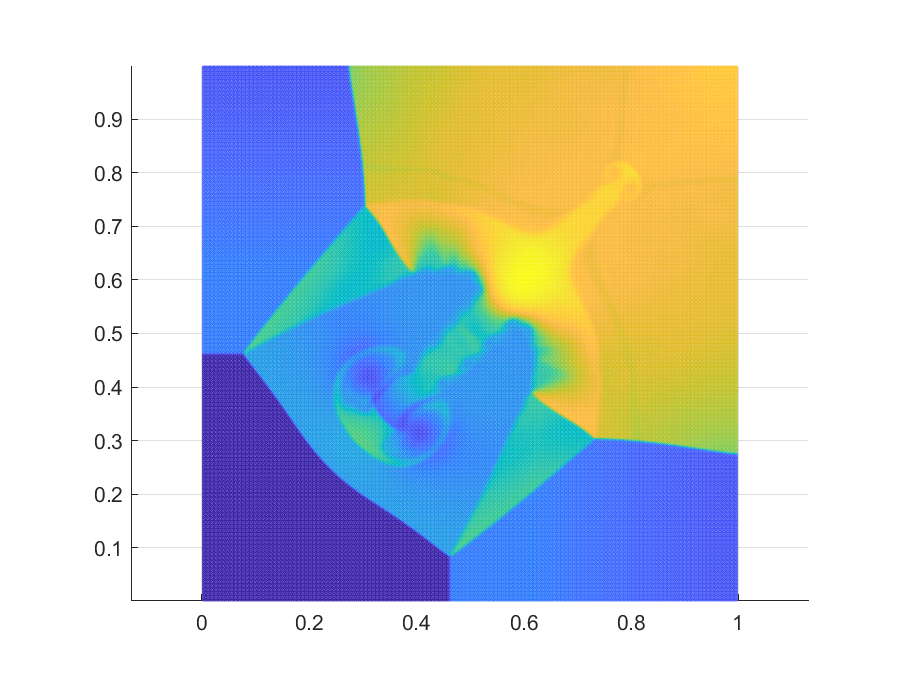
\includegraphics[width=0.45\linewidth]{fig/黎曼问题图一.eps}
        }\quad
        \subfloat{
            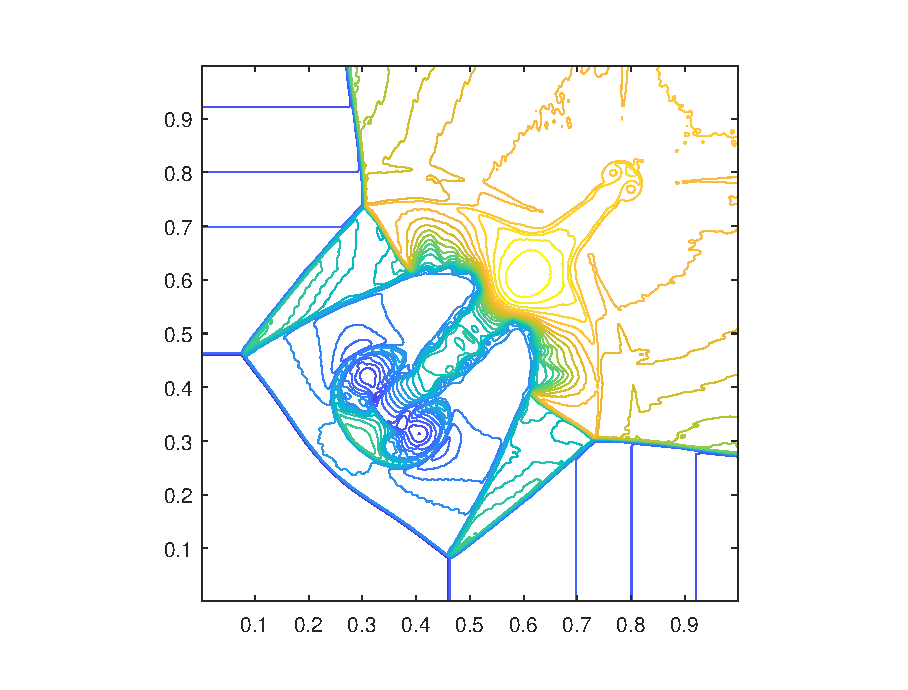
\includegraphics[width=0.45\linewidth]{fig/黎曼问题图二.eps}
        }
        \caption{WENO-JS,M=200,等高线:0.2:0.05:1.7}
    \end{figure}
\end{example}


\section{时间离散格式}
时间步长 $\Delta t$  应当满足 CFL 条件来保证稳定。对于一维标量的情况:
\begin{equation}
    \Delta t=\frac{C F L_{k} \Delta x}{\max \left|f^{\prime}(u)\right|}
\end{equation}
对于二维标量的情况:
\begin{equation}
    \Delta t=\frac{C F L_{k}}{\max \left|f^{\prime}(u)\right| / \Delta x+\max \left|g^{\prime}(u)\right| / \Delta y} .
\end{equation}
对于一维向量和二维向量的情况,上述公式中的 $\max \left|f^{\prime}(u)\right|$ 和 $\max \left|g^{\prime}(u)\right|$  被Jacobian矩阵特征值的绝对值的最大值取代. 我们使用如下的 CFL 数\cite{RN109}\cite{RN133}\cite{RN148}:  $CFL_1=0.3$, $C F L_{2}=0.18$  and  $C F L_{3}=0.1$

\subsection{ssp 二阶龙格库塔法}
ssp(strong stability-preserving)方法见:\cite{RN96}
\begin{equation}
    \begin{aligned}
        u^{(1)} & =u^{n}+\Delta t L\left(u^{n}\right)                                               \\
        u^{n+1} & =\frac{1}{2} u^{n}+\frac{1}{2} u^{(1)}+\frac{1}{2} \Delta t L\left(u^{(1)}\right)
    \end{aligned}
\end{equation}
\subsection{ssp 三阶龙格库塔法}
\begin{equation}
    \begin{aligned}
        u^{(1)} & =u^{n}+\Delta t L\left(u^{n}\right)                                                \\
        u^{(2)} & =\frac{3}{4} u^{n}+\frac{1}{4} u^{(1)}+\frac{1}{4} \Delta t L\left(u^{(1)}\right), \\
        u^{n+1} & =\frac{1}{3} u^{n}+\frac{2}{3} u^{(2)}+\frac{2}{3} \Delta t L\left(u^{(2)}\right),
    \end{aligned}
\end{equation}

\section{方程解耦}
对于双曲型方程
\begin{equation}
    \mathbf{U}_{t}+\mathbf{F}(\mathbf{U})_{x}=\mathbf{0}
\end{equation}
由链式法则可以得到:
\begin{equation}
    \mathbf{U}_{t}+\mathbf{F}_u\mathbf{U}_{x}=\mathbf{0}
\end{equation}
记 $A=F_u$,因为方程为双曲型方程,所以 $A$ 可对角化,即存在可逆矩阵 $P$ 使得
\begin{equation}
    \Lambda = P^{-1}AP
\end{equation}

\section{指示子}
指示子英文为indicator.限制器的一个重要组成部分是指示子,指示子可以找出存在强间断的小区间.
\subsection{TVB指示子}
1、基于 minmod 函数的 TVB 限制器  [6]  (简称 TVB)
\begin{equation}
    u_{i+\frac{1}{2}}^{-}=u_{i}^{(0)}+\tilde{u}_{i}, \quad u_{i-\frac{1}{2}}^{+}=u_{i}^{(0)}-\tilde{\tilde{u}}_{i}
\end{equation}
我们可以看到

\begin{equation}
    \tilde{u}_{i}=\sum_{l=1}^{k} u_{i}^{(l)} v_{l}^{(i)}\left(x_{i+\frac{1}{2}}\right), \quad \tilde{\tilde{u}}_{i}=-\sum_{l=1}^{k} u_{i}^{(l)} v_{l}^{(i)}\left(x_{i-\frac{1}{2}}\right)
\end{equation}
\begin{equation}
    \tilde{u}_{j}^{(\mathrm{mod})}=m\left(\tilde{u}_{j}, \Delta_{+} u_{j}^{(0)}, \Delta_{-} u_{j}^{(0)}\right), \quad \tilde{\tilde{u}}^{(\bmod )}=m\left(\tilde{\tilde{u}}_{j}, \Delta_{+} u_{j}^{(0)}, \Delta_{-} u_{j}^{(0)}\right),
\end{equation}
其中
\begin{equation}
    m\left(a_{1}, a_{2}, \ldots, a_{n}\right)=\begin{cases}
        a_{1}                                             & \text { if }\left|a_{1}\right| \leq M h^{2}                                                                                              \\
        s \cdot \min _{1 \leq j \leq n}\left|a_{j}\right| & \text { if } \operatorname{sign}\left(a_{1}\right)=\operatorname{sign}\left(a_{2}\right)=\cdots=\operatorname{sign}\left(a_{n}\right)=s, \\
        0                                                 & \text { otherwise }
    \end{cases}
\end{equation}



\section{限制器}
\subsection{TVB限制器}

\subsection{WENO-JS限制器}
WENO 全称为 Weighted Essentially Non-Oscillatory.WENO 限制器的思想是:使用周围的小区间上守恒量的平均值来重构当前小区间的函数,再使用得到的新函数来修正原高阶自由度,从而达到修正限制的目的.下面我们简单介绍 WENO 限制器在一维标量方程上的使用方法,一维系统的情况请参阅\cite{WENO-js1}.

\begin{enumerate}[label={{\bf Step \arabic*}:}]
    \item 首先我们在 Gauss 或 Gauss-Lobatto 积分点处重构 $u$ 的点值.对于基于 $\mathbb{P}^{k}$ 的 DG(精度为 $(k+1)$ 阶),我们需要一个至少精确到 $\mathrm{O}\left(h^{2 k+2}\right)$ 的 Gauss 或 Gauss-Lobatto 积分规则,而 WENO 重构的精度必须至少为 $2 k+1$.为此,我们需要使用相邻的 $2 k+1$ 个单元 $I_{i-k}\cdots I_{i+k}$ 的单元平均值来重构 u 的点值.
          \begin{enumerate}[label={\bf Step 1.\arabic*.}]
              \item 我们确定 $k+1$ 个小的模板 $S_{j}$,其中 $j=0,1,\cdots,k$,使得 $I_{i}$ 属于每个模板.记 $S_{j}=\cup_{l=0}^{k} I_{i+j-l}$.我们用 $\mathcal{T}=\cup_{j=0}^{k} S_{j}$ 表示包含所有 $k+1$ 个小模板的大模板.在每个模板 $S_j, j=0,\ldots,k$ 构造一个 $k$ 次多项式重构 $p_j(x)$,使得每个模板 $S_j$ 中每个单元格中 $p_j(x)$ 的平均值与给定的 $u$ 的单元格平均值相符,即\begin{equation}
                        \frac{1}{\Delta x_{i+j-l}} \int_{I_{i+j-l}} p_{j}(x) dx =u_{i+j-l}^{(0)},\quad l=0,\ldots,k.
                    \end{equation}
                    在更大的模板 $\mathcal{T}$ 上,我们再重构一个 $2k$ 次多项式 $Q(x)$,使得
                    \begin{equation}
                        \frac{1}{\Delta x_{i+l}} \int_{I_{i+l}} Q(x) dx=u_{i+l}^{(0)},\quad l=-k,\ldots,k.
                    \end{equation}
                    关于 $p_j(x)$ 和 $Q(x)$ 的构造细节可以在文献\cite{WENO5}中找到.
              \item 我们找到组合系数,也称为线性权重,记为 $\gamma_{0},\ldots,\gamma_{k}$,满足
                    \begin{equation}
                        Q(x_G)=\sum_{j=0}^k\gamma_j p_j(x_G)
                    \end{equation}
                    其中 $x_G$ 是 Gauss 积分点.不同的积分点对应不同的线性权重.
              \item 我们计算每个权重组 $S_j$ 的平滑度指示器,表示 $p_j(x)$ 在目标单元 $I_i$ 中的平滑程度.平滑度指示器 $\beta_j$ 越小,函数 $p_j(x)$ 在目标单元中的平滑度就越高,我们使用以下平滑度指示器:
                    \begin{equation}
                        \beta_{j}=\sum_{l=1}^{k} \int_{I_{i}} \Delta x_{i}^{2 l-1}\left(\frac{\partial^{l}}{\partial x^{l}} p_{j}(x)\right)^{2} d x
                    \end{equation}
              \item 我们基于平滑度指示器计算非线性权重,
                    \begin{equation}
                        \omega_{j}=\frac{\bar{\omega}_{j}}{\sum_{l} \bar{\omega}_{l}}, \quad \bar{\omega}_{j}=\frac{\gamma_{j}}{\left(\varepsilon+\beta_{j}\right)^{2}},
                    \end{equation}
                    其中,$\gamma_j$ 是在 {\bf Step 1.2.} 中确定的线性权重,$\varepsilon$ 是一个很小的数,用于避免分母为零.在本文中,我们在所有计算中使用 $\varepsilon=10^{-6}$.最终的 WENO 近似为:
                    \begin{equation}
                        u_{(x_G)} \approx \sum_{j=0}^{k} \omega_{j} p_{j}\left(x_{G}\right)
                    \end{equation}
          \end{enumerate}
    \item 基于在 Gauss 积分点 $x_G$ 上重构的点值 $u(x_G)$ 和数值积分,我们得到重构函数的高阶自由度:
          \begin{equation}
              u_{i}^{(l)}=\frac{1}{||v_{l}^{(j)}||^2} \sum_{G} w_{G} u\left(x_{G}\right) v_{l}^{(i)}\left(x_{G}\right), \quad l=1, \ldots, k
          \end{equation}
          其中,$w_{G}$ 是 Gauss 积分点 $x_{G}$ 对应的高斯积分权重.
\end{enumerate}

\begin{table}[htbp]
    \centering
    \caption{}
    \label{tab:}
    \begin{tabular}{cccccc}
        \toprule
        $x_G=x_{i+1/2}$                                                                 & $u_{i-2}^{(0)}$                     & $u_{i-1}^{(0)}$                     & $u_{i}^{(0)}$                         & $u_{i+1}^{(0)}$                     & $u_{i+2}^{(0)}$                     \\ \midrule
        $P_0(x)$                                                                        & $\frac{1}{3}$                       & $-\frac{7}{6}$                      & $\frac{11}{6}$                        &                                     &                                     \\
        $P_1(x)$                                                                        &                                     & $-\frac{1}{6}$                      & $\frac{5}{6}$                         & $\frac{1}{3}$                       &                                     \\
        $P_2(x)$                                                                        &                                     &                                     & $\frac{1}{3}$                         & $\frac{5}{6}$                       & $-\frac{1}{6}$                      \\
        $Q=\frac{1}{10}p_0+\frac{6}{10}p_1+\frac{3}{10}p_2$                             & $\frac{1}{30}$                      & $-\frac{13}{60}$                    & $\frac{47}{60}$                       & $\frac{9}{20}$                      & $-\frac{1}{20}$                     \\
        \midrule
        $x_G=x_{i+\sqrt{5}/10}$                                                         & $u_{i-2}^{(0)}$                     & $u_{i-1}^{(0)}$                     & $u_{i}^{(0)}$                         & $u_{i+1}^{(0)}$                     & $u_{i+2}^{(0)}$                     \\ \midrule
        $P_0(x)$                                                                        & $-\frac{1}{60}+\frac{\sqrt{5}}{20}$ & $\frac{1}{30}-\frac{\sqrt{5}}{5}$   & $\frac{59 }{60}+\frac{3\sqrt{5}}{20}$ &                                     &                                     \\
        $P_1(x)$                                                                        &                                     & $-\frac{1}{60}-\frac{\sqrt{5}}{20}$ & $\frac{31}{30}$                       & $-\frac{1}{60}+\frac{\sqrt{5}}{20}$ &                                     \\
        $P_2(x)$                                                                        &                                     &                                     & $\frac{59}{60}-\frac{3\sqrt{5}}{20}$  & $\frac{1}{30}+\frac{\sqrt{5}}{5}$   & $-\frac{1}{60}-\frac{\sqrt{5}}{20}$ \\
        $Q=\frac{91+9\sqrt{5}}{440}p_0+\frac{129}{220}p_1+\frac{91-9\sqrt{5}}{440}P_2 $ & $\frac{1+6\sqrt{5}}{600}$           & $-\frac{7+21\sqrt{5}}{300}$         & $\frac{313}{300}$                     & $\frac{-7+21\sqrt{5}}{300}$         & $\frac{1-6\sqrt{5}}{600}$           \\
        \bottomrule
    \end{tabular}
\end{table}

For $x_{G}=x_{i+1 / 2}$, we have
\begin{equation}
    \begin{aligned}
        p_{0}\left(x_{G}\right) & =\frac{1}{3} u_{i-2}^{(0)}-\frac{7}{6} u_{i-1}^{(0)}+\frac{11}{6} u_{i}^{(0)}                                                            \\
        p_{1}\left(x_{G}\right) & =-\frac{1}{6} u_{i-1}^{(0)}+\frac{5}{6} u_{i}^{(0)}+\frac{1}{3} u_{i+1}^{(0)},                                                           \\
        p_{2}\left(x_{G}\right) & =\frac{1}{3} u_{i}^{(0)}+\frac{5}{6} u_{i+1}^{(0)}-\frac{1}{6} u_{i+2}^{(0)},                                                            \\
        Q\left(x_{G}\right)     & =\frac{1}{30} u_{i-2}^{(0)}-\frac{13}{60} u_{i-1}^{(0)}+\frac{47}{60} u_{i}^{(0)}+\frac{9}{20} u_{i+1}^{(0)}-\frac{1}{20} u_{i+2}^{(0)},
    \end{aligned}
\end{equation}
and
\begin{equation}
    \gamma_{0}=\frac{1}{10}, \quad \gamma_{1}=\frac{6}{10}, \quad \gamma_{2}=\frac{3}{10}
\end{equation}
For  $x_{G}=x_{i+\sqrt{5} / 10}$  we have
\begin{equation}
    \begin{aligned}
        p_{0}\left(x_{G}\right) & =\left(-\frac{1}{60}+\frac{\sqrt{5}}{20}\right) u_{i-2}^{(0)}+\left(\frac{1}{30}-\frac{\sqrt{5}}{5}\right) u_{i-1}^{(0)}+\left(\frac{59}{60}+\frac{3 \sqrt{5}}{20}\right) u_{i}^{(0)},       \\
        p_{1}\left(x_{G}\right) & =\left(-\frac{1}{60}-\frac{\sqrt{5}}{20}\right) u_{i-1}^{(0)}+\frac{31}{30} u_{i}^{(0)}+\left(-\frac{1}{60}+\frac{\sqrt{5}}{20}\right) u_{i+1}^{(0)},                                        \\
        p_{2}\left(x_{G}\right) & =\left(\frac{59}{60}-\frac{3 \sqrt{5}}{20}\right) u_{i}^{(0)}+\left(\frac{1}{30}+\frac{\sqrt{5}}{5}\right) u_{i+1}^{(0)}+\left(-\frac{1}{60}-\frac{\sqrt{5}}{20}\right) u_{i+2}^{(0)},       \\
        Q\left(x_{G}\right)     & =\frac{1+6 \sqrt{5}}{600} u_{i-2}^{(0)}-\frac{7+21 \sqrt{5}}{300} u_{i-1}^{(0)}+\frac{313}{300} u_{i}^{(0)}+\frac{-7+21 \sqrt{5}}{300} u_{i+1}^{(0)}+\frac{1-6 \sqrt{5}}{600} u_{i+2}^{(0)},
    \end{aligned}
\end{equation}
and
\begin{equation}
    \gamma_{0}=\frac{91+9 \sqrt{5}}{440}, \quad \gamma_{1}=\frac{129}{220}, \quad \gamma_{2}=\frac{91-9 \sqrt{5}}{440}
\end{equation}



\chapter{更多知识}
\section{指示子}
\subsection{KXRCF指示子}
KXRCF指示子利用了DG方法的超收敛性\cite{RN92},把小单元 $I_{i,j}$ 的边界 $\partial I_{i,j}$ 分成 $\partial I_{i,j}^-,\partial I_{i,j}^+$ 两部分,分别对应流体流入和流出 $I_{i,j}$ 的边界.
\begin{equation}
    \frac{\left|\int_{\partial I_{i, j}^{-}}\left(\left.u_{h}(x, y, t)\right|_{I_{i, j}}-\left.u_{h}(x, y, t)\right|_{I_{l}}\right) d s\right|}{h_{i, j}^{R}\left|\partial I_{i, j}^{-}\right| \cdot||\mid \widehat{u_{h}}(x, y, t)|_{\partial I_{i, j}}\mid||} \geq C_{k},
\end{equation}
其中,$R=1$ 当 $k=1$, $R=1.5$ 当 $k>1$. $h_{i,j}$ 为 $I_{i,j}$ 外接圆的半径.$C_k$ 为常数,一般可取 $C_k = 1$. $I_l$ 为 $I_{i,j}$ 在 $\partial I_{i,j}^-$ 一侧的相邻单元.$u_h$ 可取守恒量,或者由守恒量引申出的物理量,$||\mid \widehat{u_{h}}(x, y, t)|_{\partial I_{i, j}}\mid||$ 为 $\mid \widehat{u_{h}}(x, y, t)|_{\partial I_{i, j}}\mid$ 在 $\partial I_{i,j}$ 上的最大值.$|\partial I_{i,j}^-|$ 为 $\partial I_{i,j}^-$ 的长度.
\section{WENO限制器}

\subsection{再看WENOJS限制器}

\subsubsection{WENOJS限制器的构造}
WENO-JS限制器首次被应用在 RKDG 上是 \cite{RKDG+WENOJS-1,RKDG+WENOJS-2}.



这里我们需要重构 $u$ 在 Gauss 或者 Gauss-Lobatto 积分点的值。对于 $\mathbb{P}^{k}$ 的 DG 方法 (具有 $k+1$ 的精度 order accurate),Gauss 或者 Gauss-Lobatto 积分规则的误差至少要达到 $\mathrm{O}\left(h^{2 k+2}\right)$。另一方面,WENO 重构多项式的精度至少要 $2 k+1$。因此,我们总共需要 $2k+1$ 个小单元上的平均值来重构 $u$ 在 Gauss 或者 Gauss-Lobatto 积分点上的值,我们使用下面的积分点:

\begin{itemize}
    \item 对于  $\mathbb{P}^{1}$  的情况, 我们使用两点高斯积分点  $x_{i-\sqrt{3} / 6}$  和  $x_{i+\sqrt{3} / 6}$ .
    \item 对于  $\mathbb{P}^{2}$  的情况, 我们使用四点 Gauss-Lobatto 积分点  $x_{i-1 / 2}, x_{i-\sqrt{5} / 10}, x_{i+\sqrt{5} / 10}$ , 和  $x_{i+1 / 2}$ .
    \item 对于  $\mathbb{P}^{3}$  的情况, 我们使用四点 Gauss 积分点  $x_{i-\sqrt{525+70 \sqrt{30}} / 70}, x_{i-\sqrt{525-70 \sqrt{30}} / 70}, x_{i+\sqrt{525-70 \sqrt{30}} / 70}$  and  $x_{i+\sqrt{525+70 \sqrt{30}} / 70}$ .
\end{itemize}

WENO最早被设计出来是作为有限差分法,有限体积法的格式用的.WENO对计算流体力学领域产生了深远的影响,在过去的几十年中,各种WENO格式的变形层出不穷,直到今天仍然有很多人在做这方面的研究.

目标是找到 $k-1$ 次多项式 $p$,满足:
\begin{equation}
    p_{i}(x)=v(x)+O\left(\Delta x^{k}\right), \quad x \in I_{i}, \quad i=1, \ldots, N
\end{equation}

考虑函数
\begin{equation}
    V(x) \equiv \int_{-\infty}^{x} v(\xi) d \xi
\end{equation}
从而
\begin{equation}
    V\left(x_{i+\frac{1}{2}}\right)=\sum_{j=-\infty}^{i} \int_{x_{j-\frac{1}{2}}}^{x_{j+\frac{1}{2}}} v(\xi) d \xi=\sum_{j=-\infty}^{i} \bar{v}_{j} \Delta x_{j}
\end{equation}
$r, s \geq 0, \text { with } r+s+1=k$
使用 $k+1$ 个点 $x_{i-r-\frac{1}{2}}, \ldots, x_{i+s+\frac{1}{2}},$ 上的 $V(x)$ 的值插值得到函数 $P(x)$, 记 $p(x)=P'(x)$,则:
\begin{equation}
    \begin{aligned}
        \frac{1}{\Delta x_{j}} \int_{x_{j-\frac{1}{2}}}^{x_{j+\frac{1}{2}}} p(\xi) d \xi & =\frac{1}{\Delta x_{j}} \int_{x_{j-\frac{1}{2}}}^{x_{j+\frac{1}{2}}} P^{\prime}(\xi) d \xi=\frac{1}{\Delta x_{j}}\left(P\left(x_{j+\frac{1}{2}}\right)-P\left(x_{j-\frac{1}{2}}\right)\right) \\
                                                                                         & =\frac{1}{\Delta x_{j}}\left(V\left(x_{j+\frac{1}{2}}\right)-V\left(x_{j-\frac{1}{2}}\right)\right)                                                                                           \\
                                                                                         & =\frac{1}{\Delta x_{j}}\left(\int_{-\infty}^{x_{j+\frac{1}{2}}} v(\xi) d \xi-\int_{-\infty}^{x_{j-\frac{1}{2}}} v(\xi) d \xi\right)                                                           \\
                                                                                         & =\frac{1}{\Delta x_{j}} \int_{x_{j-\frac{1}{2}}}^{x_{j+\frac{1}{2}}} v(\xi) d \xi=\bar{v}_{j}, \quad j=i-r, \ldots, i+s,
    \end{aligned}
\end{equation}

由数值分析可以得到:
\begin{equation}
    P^{\prime}(x)=V^{\prime}(x)+O\left(\Delta x^{k}\right), \quad x \in I_{i}
\end{equation}

在光滑的情况下,如果有:
\begin{equation}
    \omega_{r}=d_{r}+O\left(\Delta x^{k-1}\right), \quad r=0, \ldots, k-1
\end{equation}
那么:
\begin{equation}
    v_{i+\frac{1}{2}}=\sum_{r=0}^{k-1} \omega_{r} v_{i+\frac{1}{2}}^{(r)}=v\left(x_{i+\frac{1}{2}}\right)+O\left(\Delta x^{2 k-1}\right)
\end{equation}
这是因为:
\begin{equation}
    \begin{aligned}
        \sum_{r=0}^{k-1} \omega_{r} v_{i+\frac{1}{2}}^{(r)}-\sum_{r=0}^{k-1} d_{r} v_{i+\frac{1}{2}}^{(r)} & =\sum_{r=0}^{k-1}\left(\omega_{r}-d_{r}\right)\left(v_{i+\frac{1}{2}}^{(r)}-v\left(x_{i+\frac{1}{2}}\right)\right) \\
                                                                                                           & =\sum_{r=0}^{k-1} O\left(\Delta x^{k-1}\right) O\left(\Delta x^{k}\right)=O\left(\Delta x^{2 k-1}\right)
    \end{aligned}
\end{equation}
$\beta_{r}$  被称为模板  $S_{r}(i)$ 的光滑指示器 "smooth indicators" .如果 $v(x)$ 在模板 $S_{r}(i) $ 是光滑的,那么:
\begin{equation}
    \beta_{r}=O\left(\Delta x^{2}\right)
\end{equation}
但是如果 $v(x)$ 在模板 $S_{r}(i) $ 有间断,那么:
\begin{equation}
    \beta_{r}=O(1)
\end{equation}
对应到非线性权,当 $v(x)$ 在模板 $S_{r}(i) $ 是光滑的,那么:
\begin{equation}
    \omega_{r}=O\left(\Delta x^{4}\right)
\end{equation}
但是如果 $v(x)$ 在模板 $S_{r}(i) $ 有间断,那么:
\begin{equation}
    \omega_{r}=O(1)
\end{equation}

One also has to worry about the accuracy requirement  (2.56) , which must be checked when the specific form of the smooth indicator  $\beta_{r}$  is given. For any smooth indicator  $\beta_{r}$ , it is easy to see that the weights defined by (2.58) satisfies (2.53). To satisfy (2.56), it suffices to have, through a Taylor expansion analysis:

\begin{equation}
    \beta_{r}=D\left(1+O\left(\Delta x^{k-1}\right)\right), \quad r=0, \ldots, k-1
\end{equation}

where  $D$  is a nonzero quantity independent of  $r$  (but may depend on  $\Delta x$  ).

WENO-M限制器在文章\cite{WENO-M}中被提出,在该文章中.作者详细分析了 WENO 实现预期精度的的充要条件,并且指出 WENO-JS 格式会在 critical points 附近会损失精度,但是由于 $\epsilon$,这一特点没有在WENO-JS中被发现,并且给出了一个新的格式 MWENO 克服了这一问题.

\begin{equation}
    \omega_{k}^{(\mathrm{JS})}=\frac{\alpha_{k}}{\sum_{i=0}^{2} \alpha_{i}}, \quad \text { where } \alpha_{k}=\frac{\bar{\omega}_{k}}{\left(\epsilon+\beta_{k}\right)^{p}},
\end{equation}

为了满足五阶格式的要求,需要满足以下充要条件:
\begin{subequations}
    \begin{align}
        \sum_{k=0}^{2}\left(\omega_{k}-\bar{\omega}_{k}\right)=\mathrm{O}\left(\Delta x^{6}\right),                                                                \\
        \left(3 \omega_{1}^{(+)}-3 \omega_{1}^{(-)}-\omega_{2}^{(+)}+\omega_{2}^{(-)}+\omega_{3}^{(+)}-\omega_{3}^{(-)}\right)=\mathrm{O}\left(\Delta x^{3}\right) \\
        \left(\omega_{k}-\bar{\omega}_{k}\right)=\mathrm{O}\left(\Delta x^{2}\right)
    \end{align}
\end{subequations}

假如光滑指示器可以写成下面的形式:
\begin{equation}
    \beta_{k}=D\left(1+\mathrm{O}(\Delta x)^{2}\right)
\end{equation}
其中 $D$ 是一些与 $k$ 无关的非零常数

\begin{equation}
    \bar{\omega}_{k}=\frac{\gamma_k}{\left(D\left(1+\mathrm{O}(\Delta x)^{2}\right)\right)^{p}}=\frac{\gamma_k}{D^{p}}\left(1+\mathrm{O}\left(\Delta x^{2}\right)\right)
\end{equation}
\begin{equation}
    \sum_{k=0}^{2} \alpha_{k}=\frac{1}{D^{p}}\left(1+\mathrm{O}\left(\Delta x^{2}\right)\right)
\end{equation}


taking into account that  $\sum_{k=0}^{2} \bar{\omega}_{k}=1$ . Thus $ \omega_{k}^{(\mathrm{JS})}$ , as defined in Eq. (30), is given by
\begin{equation}
    \omega_{k}^{(\mathrm{JS})}=\bar{\omega}_{k}+\mathrm{O}\left(\Delta x^{2}\right)
\end{equation}
which agrees with Eq. (29c). Note that Eq. (29b) is still not satisfied by enforcing Eq. (31).


\begin{subequations}
    \begin{align}
        \beta_{0} & =\frac{13}{12}\left(f_{i-2}-2 f_{i-1}+f_{i}\right)^{2}+\frac{1}{4}\left(f_{i-2}-4 f_{i-1}+3 f_{i}\right)^{2},  \\
        \beta_{1} & =\frac{13}{12}\left(f_{i-1}-2 f_{i}+f_{i+1}\right)^{2}+\frac{1}{4}\left(f_{i-1}-f_{i+1}\right)^{2},            \\
        \beta_{2} & =\frac{13}{12}\left(f_{i}-2 f_{i+1}+f_{i+2}\right)^{2}+\frac{1}{4}\left(3 f_{i}-4 f_{i+1}+f_{i+2}\right)^{2} .
    \end{align}
\end{subequations}

\begin{subequations}
    \begin{align}
        \beta_{0} & =f_{i}^{\prime 2} \Delta x^{2}+\left(\frac{13}{12} f_{i}^{\prime \prime 2}-\frac{2}{3} f_{i}^{\prime} f_{i}^{\prime \prime \prime}\right) \Delta x^{4}-\left(\frac{13}{6} f_{i}^{\prime \prime} f_{i}^{\prime \prime \prime}-\frac{1}{2} f_{i}^{\prime} f_{i}^{\prime \prime \prime \prime}\right) \Delta x^{5}+\mathrm{O}\left(\Delta x^{6}\right),  \\
        \beta_{1} & =f_{i}^{\prime 2} \Delta x^{2}+\left(\frac{13}{12} f_{i}^{\prime \prime 2}+\frac{1}{3} f_{i}^{\prime} f_{i}^{\prime \prime \prime}\right) \Delta x^{4}+\mathrm{O}\left(\Delta x^{6}\right),                                                                                                                                                           \\
        \beta_{2} & =f_{i}^{\prime 2} \Delta x^{2}+\left(\frac{13}{12} f_{i}^{\prime \prime 2}-\frac{2}{3} f_{i}^{\prime} f_{i}^{\prime \prime \prime}\right) \Delta x^{4}+\left(\frac{13}{6} f_{i}^{\prime \prime} f_{i}^{\prime \prime \prime}-\frac{1}{2} f_{i}^{\prime} f_{i}^{\prime \prime \prime \prime}\right) \Delta x^{5}+\mathrm{O}\left(\Delta x^{6}\right) .
    \end{align}
\end{subequations}


\subsubsection{WENO-JS的局限性}
\begin{itemize}
    \item 对于非结构化网络,需要计算线性权重,计算较为繁琐
    \item 耗散较大,捕捉细小尺度的流动结构不够精确
    \item 需要用到的模板较大,紧致性差(破坏了DG方法的紧致性).
    \item 在部分光滑情况下存在丢精度的可能.
\end{itemize}
\subsection{修改光滑指示器(Smoothness indicators)}
\subsubsection{WENO-Z}
在WENO-Z方案中,非归一化和归一化非线性权重$\alpha_{k}^{Z}$和$\omega_{k}^{Z}$的一般定义分别为:
\begin{equation}
    \alpha_{k}^{\mathrm{Z}}=d_{k}\left[1+\left(\frac{\tau}{\beta_{k}+\varepsilon}\right)^{p}\right], \quad \omega_{k}^{\mathrm{z}}=\frac{\alpha_{k}^{\mathrm{z}}}{\sum_{j=0}^{r-1} \alpha_{j}^{\mathrm{z}}}, \quad k=0, \ldots, r-1 .
\end{equation}
与 WENO-JS 权重一样,$p$ 和 $\varepsilon$ 分别是power和sensitivity参数。 它们类似于 WENO-JS 方案中的参数。

WENO-Z 方案相对于经典方案的新颖思想是在非线性权重的形成中包含从全局阶平滑度指标 $\tau$ 获得的高阶信息。 这个全局平滑度指标是 $\beta_{k}$ 的线性组合,即:
\begin{equation}
    \tau=\left|\sum_{k=0}^{r-1} c_{k} \beta_{k}\right|
\end{equation}
其中 $c_{k}$ 是给定的常量。例如,五阶WENO-Z方案的$\tau$的表达式为:
\begin{equation}
    \tau=\left|\beta_{0}-\beta_{2}\right| .
\end{equation}
$\tau$ 的顺序随 $R$ 的变化而变化; 对于五阶 WENO-Z,它的阶数恰好也是 5.更多的 $\tau$ 的定义可查看表格\cite{WENO-Z-2013}
\begin{table}[htbp]
    \centering
    \label{table:tau_ref}
    \caption{The global optimal order smoothness indicator  $\tau_{2 r-1}$  and its leading truncation order  $\theta\left(\tau_{2 r-1}\right)$  of the  $(2 r-1)$  order WENO-Z scheme.}
    \begin{tabular}{cccc}
        \toprule
        $r$ & $2r-1$ & $\tau_{2r-1}$                                                 & $\theta(\tau_{2r-1})$ \\
        \midrule
        2   & 3      & $|\beta_0-\beta_1|$                                           & 3                     \\
        3   & 5      & $|\beta_0-\beta_2|$                                           & 5                     \\
        4   & 7      & $|\beta_0+3\beta_1-3\beta_2-\beta_3|$                         & 7                     \\
        5   & 9      & $|\beta_0+2\beta_1-6\beta_2+2\beta_3+\beta_4|$                & 8                     \\
        6   & 11     & $|\beta_0+\beta_1-8\beta_2+8\beta_3-\beta_4-\beta_5|$         & 9                     \\
        7   & 13     & $|\beta_0+36\beta_1+135\beta_2-135\beta_4-36\beta_5-\beta_6|$ & 11                    \\
        \bottomrule
    \end{tabular}
\end{table}

和WENO-JS相同,  $\varepsilon$  对 WENO-Z 的精度有影响; 但是不同于 WENO-JS, $\varepsilon$ 上的条件随 $R$ 和 $p$ 变化并且较弱. 例如, 在  $R=5$  且  $p=2$ 的情况下, 如果 $ \varepsilon=\Omega\left(\Delta x^{4}\right)$,WENO-Z 实现5阶精度, 但是对于  $\varepsilon<\mathrm{O}\left(\Delta x^{4}\right)$  精度通常会在接近 2 阶临界点时降低.
\begin{equation}
    \tau_{5}=\left|\beta_{0}-\beta_{2}\right|=\frac{13}{3}\left|f_{i}^{\prime \prime} f_{i}^{\prime \prime \prime}\right| \Delta x^{5}+\mathrm{O}\left(\Delta x^{6}\right)
\end{equation}
假设在模板 2 中存在间断,那么 $\beta_2>\beta_k$,从而:
\begin{equation}
    \frac{\beta_{k}^{z}}{\beta_{2}^{z}}=\frac{\beta_{k}}{\beta_{2}} \frac{\beta_{2}+\tau_{5}}{\beta_{k}+\tau_{5}} \geqslant \frac{\beta_{k}}{\beta_{2}}, \quad k=0,1,
\end{equation}
所以,相比于 WENO-JS, WENO-Z 会增加间断模板的权重.作者认为,WENO-Z 耗散更小的原因就在于此。

\subsection{自由设置线性权}

\subsubsection{MRWENO}
朱军等人在一列论文\cite{MRWENO-1,MRWENO-2,MRWENO-3}中发展了 MRWENO(multi-resolution WENO)限制器。
\begin{enumerate}[label={{\bf Step \arabic*}:}]
    \item 1
          \begin{enumerate}[label={\bf Step 1.\arabic*.}]
              \item 在有问题的单元 $I_j$ 上定义一系列不同次数的多项式.我们构造多项式 $q_{\ell}(x), \ell=0, \ldots, k$,满足以下条件:
                    \begin{equation}
                        \int_{I_j} q_{\ell}(x) v_{l}^{j}(x) \dd x=\int_{I_j} u_{h}(x) v_{l}^{j}(x, y) \dd x,\, l=0,1, \ldots, \ell.
                    \end{equation}
                    \begin{remark}
                        如果我们采用规范正交基 $v_{l}^{(0)}(x)$,那么不同的多项式 $q_{\ell}(x), \ell=0,1, \ldots, k$ 的构造非常简单.在这种情况下,我们可以直接得到多项式
                        \begin{equation}
                            q_{\ell}(x)=\sum_{l=0}^{\ell} u_{j}^{(l)}(t) v_{l}^{(j)}(x),\,\ell=0,1,\ldots, k.
                        \end{equation}
                    \end{remark}
              \item 我们通过以下方式构造多项式 $p_{\ell, \ell}(x),p_{\ell,\ell+1} \ell(x)=1, \ldots, k$
                    \begin{equation}
                        p_{\ell, \ell}(x)=\frac{1}{\gamma_{\ell, \ell}} q_{\ell}(x)-\frac{\gamma_{\ell-1, \ell}}{\gamma_{\ell, \ell}} p_{\ell-1, \ell}(x), \ell=1, \ldots, k,
                    \end{equation}
                    \begin{equation}
                        p_{\ell, \ell+1}(x)=\omega_{\ell, \ell} p_{\ell, \ell}(x)+\omega_{\ell-1, \ell} p_{\ell-1, \ell}(x), \ell=1, \ldots, k-1
                    \end{equation}
                    这些表达式中,$\gamma_{\ell-1, \ell}$ 和 $\gamma_{\ell, \ell}$ 是线性权重,要求 $\gamma_{\ell-1, \ell}+\gamma_{\ell, \ell}=1$,且 $\gamma_{\ell-1, \ell},\gamma_{\ell, \ell}>0$.由于对于平滑解来说,高阶解通常是最好的,因此我们给予高阶多项式更高的线性权重,基于低阶多项式更小的线性权重.即:
                    \begin{equation}
                        \gamma_{\ell_,\ell} \gg \gamma_{\ell-1,\ell}
                    \end{equation}
                    当比值 $\frac{\gamma_{\ell_,\ell}}{\gamma_{\ell-1,\ell}}$ 的值较小时,可以在不连续性上获得更好的结果,而当值较大时,通常对于平滑解更好.在我们的数值测试中,我们取
                    \begin{equation}
                        \gamma_{\ell-1, \ell}=0.01,\quad  \gamma_{\ell, \ell}=0.99,\quad \ell=1, \ldots, k
                    \end{equation}
                    这可以在平滑区域中保持原始的高阶,在所有数值例子中都可以保持基本上非振荡的冲击过渡.

                    $\omega_{\ell-1, \ell}$ 和 $\omega_{\ell, \ell}$ 是非线性权重(稍后将准确地介绍).
              \item 计算光滑指示器  $\beta_{\ell, \ell_{2}}$ , 其衡量了  $p_{\ell, \ell_{2}}(x, y)$  for  $\ell=\ell_{2}-1 ,  \ell_{2} ; \ell_{2}=1,2,3,4$  在小区间  $I_{j}$ 上的光滑程度. 具体来说:$\beta_{\ell, \ell_{2}}$ 越小,说明 $p_{\ell, \ell_{2}}(x, y)$ 在 $I_{j}$ 上越光滑.
                    \begin{equation}
                        \label{eqa:光滑指示器}
                        \beta_{l_1,l_2}=\sum_{l=1}^{k} \int_{I_{i}} \Delta x_{i}^{2 l-1}\left(\frac{\partial^{l}}{\partial x^{l}} p_{l_1,l_2}(x)\right)^{2} d x
                    \end{equation}
                    由于 $p_{0,1}(x)$ 是一个常值函数,$p'_{0,1}(x)=0$,因此无法使用统一的\eqref{eqa:光滑指示器}式来衡量其光滑程度,因此我们为 $p_{0,1}(x)$ 设计了其独有的限制器:

                    定义线性函数 $q_{0,1}(x),q_{0,2}(x)$ 满足:

                    \begin{equation}
                        \begin{aligned}
                            \int_{I_{j-1}}q_{0,1}(x)v_{l}^{(j-1)}(x)\dd x & = \int_{I_{j-1}}u_h(x)v_{l}^{(j-1)}\dd x,\quad l=0,1,\cdots,k \\
                            \int_{I_{j+1}}q_{0,1}(x)v_{l}^{(j+1)}(x)\dd x & = \int_{I_{j+1}}u_h(x)v_{l}^{(j+1)}\dd x,\quad l=0,1,\cdots,k \\
                        \end{aligned}
                    \end{equation}
                    再构造 $\varsigma_1,\varsigma_2$,其定义如下:
                    \begin{equation}
                        \varsigma_1=\int_{I_{j}}\left(\frac{\dd}{\dd x}q_{0,1}\right)^2\dd x,\quad \varsigma_2=\int_{I_{j}}\left(\frac{\dd}{\dd x}q_{0,1}\right)^2\dd x\\
                    \end{equation}
                    $\beta_{0,1}$ 定义取 $\varsigma_1,\varsigma_2$ 的最小值:
                    \begin{equation}
                        \beta_{0,1} = \min\{\varsigma_1,\varsigma_2 \}.
                    \end{equation}
              \item    基于线性权重和光滑性指标计算非线性权重.我们采用文献\cite{WENO-Z} 中所示的WENO-Z的做法,$\tau_{\ell_{2}}$ 定义如下:
                    \begin{equation}
                        \tau_{\ell_2} = (\beta_{\ell_2,\ell_2}-\beta_{\ell_2-1,\ell_2})^2
                    \end{equation}
                    \begin{equation}
                        \omega_{\ell_{1}, \ell_{2}}=\frac{\bar{\omega}_{\ell_{1}, \ell_{2}}}{\sum_{\ell=\ell_{2}-1}^{\ell_{2}} \bar{\omega}_{\ell, \ell_{2}}},\quad \bar{\omega}_{\ell_{1}, \ell_{2}}=\gamma_{\ell_{1},\ell_{2}}\left(1+\frac{\tau_{\ell_2}}{\epsilon+\beta_{\ell_1,\ell_2}}\right)
                    \end{equation}
                    得到最终的拟合函数:
                    \begin{equation}
                        p^{\text {new }}(x)=\sum_{\ell=\ell_{2}-1}^{\ell_{2}} \omega_{\ell, \ell_{2}} p_{\ell, \ell_{2}}(x), \quad \ell_{2}=1,2,3,4,
                    \end{equation}
                    \begin{equation}
                        u_{j}^{(l)}(t)=\frac{1}{||v_{l}^{(j)}||^{2}} \int_{I_{j}} u(x, t) v_{l}^{(j)}(x) d x, \quad l=0,1,\cdots, k .
                    \end{equation}
          \end{enumerate}
    \item 修正高阶矩
\end{enumerate}


\begin{remark}
    如果不修正线性权重,那么最终会得到 $p^{\text {new }}(x)=p^{\text {old }}(x)$.
    \begin{equation}
        \begin{aligned}
            p^{\text {new }}(x) & =\gamma_{l_1,l_2}p_{l_1,l_2}(x)+\gamma_{l_2,l_2}p_{l_2,l_2}(x)                                                                                            \\
                                & =\gamma_{l_1,l_2}p_{l_1,l_2}(x)+\gamma_{l_2,l_2}\left(\frac{1}{\gamma_{l_2,l_2}}q_{l_2}(x)-\frac{\gamma_{l_1,l_2}}{\gamma_{l_2,l_2}}p_{l_1,l_2}(x)\right) \\
                                & =q_{l_2}(x)=p^{\text {old }}(x)
        \end{aligned}
    \end{equation}
\end{remark}

\begin{equation}
    \beta_{\ell, \ell_{2}}=\sum_{|\alpha|=1}^{\kappa} \int\left(\Delta x_{i} \Delta y_{j}\right)^{|\alpha|-1}\left(\frac{\partial^{|\alpha|}}{\partial x^{\alpha_{1}} \partial y^{\alpha_{2}}} p_{\ell, \ell_{2}}(x, y)\right)^{2} d x d y
\end{equation}


特别的:
\begin{equation}
    \begin{aligned}
        p_{01} & = q_0                                                             \\
        p_{11} & = \frac{1}{\gamma_{11}}q_1-\frac{\gamma_{01}}{\gamma_{11}}p_{01}  \\
        p_{12} & =\omega_{11}p_{11} + \omega_{01}p_{0,1}                           \\
        p_{22} & =\frac{1}{\gamma_{22}}q_2 - \frac{\gamma_{12}}{\gamma_{22}}p_{12} \\
    \end{aligned}
\end{equation}

\begin{equation}
    \begin{aligned}
        p^{\text {MR-WENO2 }}(x, y, z) & =\omega_{0,1} p_{0,1}(x, y, z)+\omega_{1,1} p_{1,1}(x, y, z),          \\
        p^{\text{MR-WENO3}}(x, y, z)   & =\omega_{1,2} p^{M R-W E N O 2}(x, y, z)+\omega_{2,2} p_{2,2}(x, y, z)
    \end{aligned}
\end{equation}

一维时:
\begin{equation}
    \begin{aligned}
        \beta_{01} & = 4\,{a_1 }^2                                                                                                                                                                                                                                                                 \\
        \beta_{11} & = \frac{4\,{a_1 }^2 }{{\gamma_{11} }^2 }                                                                                                                                                                                                                                      \\
        \beta_{12} & = \frac{4\,{a_1 }^2 \,{\omega_{11} }^2 }{{\gamma_{11} }^2 }                                                                                                                                                                                                                   \\
        \beta_{22} & = \frac{144\,{a_2 }^2 }{{\gamma_{22} }^2 }+\frac{4\,{\left({a_1 }^2 \,{\gamma_{11} }^2 -2\,{a_1 }^2 \,\gamma_{11} \,\gamma_{12} \,\omega_{11} +{a_1 }^2 \,{\gamma_{12} }^2 \,{\omega_{11} }^2 +3\,{a_2 }^2 \,{\gamma_{11} }^2 \right)}}{{\gamma_{11} }^2 \,{\gamma_{22} }^2 } \\
    \end{aligned}
\end{equation}
二维时:
\begin{equation}
    \begin{aligned}
        \beta_{01} & = {\left(\mathrm{xa}-\mathrm{xb}\right)}\,{\left(\mathrm{ya}-\mathrm{yb}\right)}\,{\left(\frac{4\,{a_1 }^2 }{{{\left(\mathrm{xa}-\mathrm{xb}\right)}}^2 }+\frac{4\,{a_2 }^2 }{{{\left(\mathrm{ya}-\mathrm{yb}\right)}}^2 }\right)}                                                                                                                                                                                \\
        \beta_{11} & = {\left(\frac{4\,{a_1 }^2 }{{\gamma_{11} }^2 \,{{\left(\mathrm{xa}-\mathrm{xb}\right)}}^2 }+\frac{4\,{a_2 }^2 }{{\gamma_{11} }^2 \,{{\left(\mathrm{ya}-\mathrm{yb}\right)}}^2 }\right)}\,{\left(\mathrm{xa}-\mathrm{xb}\right)}\,{\left(\mathrm{ya}-\mathrm{yb}\right)}                                                                                                                                          \\
        \beta_{12} & = \frac{{a_1 }^2 \,{\omega_{11} }^2 \,{\left(\mathrm{xa}-\mathrm{xb}\right)}\,{\left(\mathrm{ya}-\mathrm{yb}\right)}}{{\gamma_{11} }^2 \,{{\left(\frac{\mathrm{xa}}{2}-\frac{\mathrm{xb}}{2}\right)}}^2 }+\frac{{a_2 }^2 \,{\omega_{11} }^2 \,{\left(\mathrm{xa}-\mathrm{xb}\right)}\,{\left(\mathrm{ya}-\mathrm{yb}\right)}}{{\gamma_{11} }^2 \,{{\left(\frac{\mathrm{ya}}{2}-\frac{\mathrm{yb}}{2}\right)}}^2 } \\
    \end{aligned}
\end{equation}
$\beta_{22}$ 太复杂了,单独写一下
\begin{equation}
    \begin{aligned}
        \beta_{22} = & \frac{4\,{\left(\mathrm{ya}-\mathrm{yb}\right)}\,{\left(3\,{a_1 }^2 \,{\gamma_{11} }^2 -6\,{a_1 }^2 \,\gamma_{11} \,\gamma_{12} \,\omega_{11} +3\,{a_1 }^2 \,{\gamma_{12} }^2 \,{\omega_{11} }^2 +4\,{a_3 }^2 \,{\gamma_{11} }^2 +{a_5 }^2 \,{\gamma_{11} }^2 \right)}}{3\,{\gamma_{11} }^2 \,{\gamma_{22} }^2 \,{\left(\mathrm{xa}-\mathrm{xb}\right)}}  \\
                     & +\frac{4\,{\left(\mathrm{xa}-\mathrm{xb}\right)}\,{\left(3\,{a_2 }^2 \,{\gamma_{11} }^2 -6\,{a_2 }^2 \,\gamma_{11} \,\gamma_{12} \,\omega_{11} +3\,{a_2 }^2 \,{\gamma_{12} }^2 \,{\omega_{11} }^2 +4\,{a_4 }^2 \,{\gamma_{11} }^2 +{a_5 }^2 \,{\gamma_{11} }^2 \right)}}{3\,{\gamma_{11} }^2 \,{\gamma_{22} }^2 \,{\left(\mathrm{ya}-\mathrm{yb}\right)}} \\
                     & +\frac{64\,{a_3 }^2 \,{{\left(\mathrm{ya}-\mathrm{yb}\right)}}^2 }{{\gamma_{22} }^2 \,{{\left(\mathrm{xa}-\mathrm{xb}\right)}}^2 } + \frac{64\,{a_4 }^2 \,{{\left(\mathrm{xa}-\mathrm{xb}\right)}}^2 }{{\gamma_{22} }^2 \,{{\left(\mathrm{ya}-\mathrm{yb}\right)}}^2 }+\frac{16\,{a_5 }^2 }{{\gamma_{22} }^2 }
    \end{aligned}
\end{equation}

事实上,所谓的自由设置线性权也不是完全自由。如果给定一个比较差的线性权,是无法重构到原精度的。数值例子可见 \cite{RN133}

\subsection{HWENO}




\section{保极值限制器}
% https://zhuanlan.zhihu.com/p/539865055
% https://zhuanlan.zhihu.com/p/542538581
\subsection{一维}
\cite{RN6}
标量守恒性方程
\begin{equation}
    u_{t}+\nabla \cdot \mathbf{F}(u)=0 \quad \text { and } \quad u(\mathbf{x}, 0)=u_{0}(\mathbf{x})
\end{equation}
一个很重要的性质就是它满足最大值原则.具体来说,如果 $M=\max_x u_0(x)$,$m=\min_x u_0(x)$, 那么 $u(x,t)\in[m,M]$. 对任意的 $x,t$ 都满足.所以,我们也希望数值解也满足这个性质.因为在一些情况下,超出了这个范围,就会得到无物理意义的解.比如负密度,或者负百分比,或者某个多组分混合物中某个组分的百分比大于一.这样的限制器在多项流问题中尤为重要.\cite{PP-review}

证明的思路为:首先证明当时间步长充分小的时候一阶格式下是保界的,然后证明在步长充分小的时候高阶格式的单元平均值是保界的,然后对高阶格式的 $u_h-\bar{u}_h$ 做一个简单的线性限制,使得高阶格式也能保界。

\begin{theorem}
    对于一阶(单调monotone)格式
    \begin{equation}
        u_{j}^{n+1}=u_{j}^{n}-\lambda\left[\hat{f}\left(u_{j}^{n}, u_{j+1}^{n}\right)-\hat{f}\left(u_{j-1}^{n}, u_{j}^{n}\right)\right] \equiv H_{\lambda}\left(u_{j-1}^{n}, u_{j}^{n}, u_{j+1}^{n}\right),
    \end{equation}
    满足严格的极值原则,其中 $\lambda=\Delta t / \Delta x$,$\Delta t$  和  $\Delta x$ 分别为时间步长和空间步长,并且$\hat{f}(a, b)$ 是 monotone 通量,满足三条件。即:当
    \begin{equation}
        \label{eqa:pp_1D_1Order_CFL}
        \alpha \lambda \leq 1, \quad \alpha=\max \left|f^{\prime}(u)\right|,
    \end{equation}
    时,如果有:$m \leq u_{j-1}^{n}, u_{j}^{n}, u_{j+1}^{n} \leq M .$,那么有 $u_{j}^{n+1}\in[m,M]$。
\end{theorem}
\begin{proof}
    对于 Lax-Friedrichs 结构 和 Godunov 结构
    可以证明 $H_{\lambda}(a, b, c)$  对于三个变量都是单调递增的,且一致的,即: $H_{\lambda}(a, a, a)=a$. 在这种情况下:
    \begin{equation}
        m=H_{\lambda}(m, m, m) \leq u_{j}^{n+1}=H_{\lambda}\left(u_{j-1}^{n}, u_{j}^{n}, u_{j+1}^{n}\right) \leq H_{\lambda}(M, M, M)=M
    \end{equation}
    对于其他结构,我没有在\cite{PP-review}中找到证明。
\end{proof}
下面考虑对于一般的高阶格式
\begin{equation}
    \label{eqa:pp_high_order_scheme}
    \begin{aligned}
        \bar{u}_{j}^{n+1} & =\bar{u}_{j}^{n}-\lambda\left[\hat{f}\left(u_{j+1 / 2}^{-}, u_{j+1 / 2}^{+}\right)-\hat{f}\left(u_{j-1 / 2}^{-}, u_{j-1 / 2}^{+}\right)\right] \\
                          & \equiv G_{\lambda}\left(\bar{u}_{j}^{n}, u_{j+1 / 2}^{-}, u_{j+1 / 2}^{+}, u_{j-1 / 2}^{-}, u_{j-1 / 2}^{+}\right)
    \end{aligned}
\end{equation}
中的单元平均值的保界性。考虑$I_{j}=\left[x_{j-1 / 2}, x_{j+1 / 2}\right]$ 上的 $n$ 点的 Gauss-Lobatto 高斯点,其对于阶数小于等于 $2N-3$ 的多项式的数值积分是准确的。我们将这些 $I_{j}$ 上的积分点记作:
\begin{equation}
    S_{j}=\left\{x_{j-1 / 2}=\hat{x}_{j}^{1}, \hat{x}_{j}^{2}, \ldots, \hat{x}_{j}^{N-1}, \hat{x}_{j}^{N}=x_{j+1 / 2}\right\} .
\end{equation}
记 $\hat{w}_{\alpha}$ 为 $\left[-\frac{1}{2}, \frac{1}{2}\right]$ 上的Gauss-Lobatto的权重,从而:$\sum_{\alpha=1}^{N} \hat{w}_{\alpha}=1$,$N$ 为满足 $2 N-3 \geqslant k$ 的最小整数.那么:
\begin{equation}
    \label{eqa:pp_ave_u}
    \bar{u}_{j}^{n}=\frac{1}{\Delta x} \int_{I_{j}} p_{j}(x) \mathrm{d} x=\sum_{\alpha=1}^{N} \hat{w}_{\alpha} p_{j}\left(\hat{x}_{j}^{\alpha}\right)=\sum_{\alpha=2}^{N-1} \hat{w}_{\alpha} p_{j}\left(\hat{x}_{j}^{\alpha}\right)+\hat{w}_{1} u_{j-1 / 2}^{+}+\hat{w}_{N} u_{j+1 / 2}^{-} .
\end{equation}
$p_j$ 表示第 $j$ 个小单元上的多项式,$u_{j-1/2}^+=p_j(x_{j-1/2})$, $u_{j+1/2}^-=p_j(x_{j+1/2})$
\begin{theorem}{}{}
    如果 $u_{j-1/2}^-$, $u_{j+1/2}^+$, $p_j(\hat{x}_j^\alpha)(\alpha=1,2,\cdots,N)\in[m,M]$,且在CFL条件
    \begin{equation}
        \lambda a \leq \hat{w}_{1}
    \end{equation}
    满足的条件下,$\bar{u}_j^{n+1}\in[m,M]$.
\end{theorem}
\begin{proof}
    将等式 \eqref{eqa:pp_ave_u} 带入 \eqref{eqa:pp_high_order_scheme} 中, 再增减  $\hat{f}\left(u_{j-1 / 2}^{+}, u_{j+1 / 2}^{-}\right)$ , \eqref{eqa:pp_high_order_scheme} 可变为:
    \begin{equation}
        \begin{aligned}
            \bar{u}_{j}^{n+1}= & \sum_{\alpha=2}^{N-1} \hat{w}_{\alpha} p_{j}\left(\hat{x}_{j}^{\alpha}\right)+\hat{w}_{N}\left(u_{j+1 / 2}^{-}-\frac{\lambda}{\hat{w}_{N}}\left[\hat{f}\left(u_{j+1 / 2}^{-}, u_{j+1 / 2}^{+}\right)-\hat{f}\left(u_{j-1 / 2}^{+}, u_{j+1 / 2}^{-}\right)\right]\right) \\
                               & +\hat{w}_{1}\left(u_{j-1 / 2}^{+}-\frac{\lambda}{\hat{w}_{1}}\left[\hat{f}\left(u_{j-1 / 2}^{+}, u_{j+1 / 2}^{-}\right)-\hat{f}\left(u_{j-1 / 2}^{-}, u_{j-1 / 2}^{+}\right)\right]\right)                                                                              \\
            =                  & \sum_{\alpha=2}^{N-1} \hat{w}_{\alpha} p_{j}\left(\hat{x}_{j}^{\alpha}\right)+\hat{w}_{N} H_{\lambda / \hat{\omega}_{N}}\left(u_{j-1 / 2}^{+}, u_{j+1 / 2}^{-}, u_{j+1 / 2}^{+}\right)                                                                                  \\
                               & +\hat{w}_{1} H_{\lambda / \hat{\omega}_{1}}\left(u_{j-1 / 2}^{-}, u_{j-1 / 2}^{+}, u_{j+1 / 2}^{-}\right) .
        \end{aligned}
    \end{equation}
    注意到  $\hat{w}_{1}=\hat{w}_{N}$,并且 $H_{\lambda / \hat{\omega}_{1}}$  在CFL条件\eqref{eqa:pp_1D_1Order_CFL}下是单调的,所以从上式中可以看出 $\bar{u}_{j}^{n+1}$  对于所有包含的变量$u_{j-1 / 2}^{-}, u_{j+1 / 2}^{+}$ and  $p_{j}\left(\hat{x}_{j}^{\alpha}\right)$  for  $1 \leq j \leq N$ 都是单调增加的.

    下面这句话很奇怪没有看懂:

    (The same proof for the first-order monotone scheme now applies to imply  $\bar{u}_{j}^{n+1} \in[m, M])$.
\end{proof}

对高阶矩的限制比较简单,只是做了一个线性限制器,重要的是限制之后的多项式没有损失原有的精度。

\begin{remark}
    这个留到下次再写
\end{remark}
\subsection{二维}
先来说明小单元为矩阵的情况:

对于二维的情况:
\begin{equation}
    \begin{aligned}
        \bar{u}_{i j}^{n+1}= & \bar{u}_{i j}^{n}-\frac{\Delta t}{\Delta x \Delta y} \int_{y_{j-1 / 2}}^{y_{j+1 / 2}} \hat{f}\left[u_{i+1 / 2, j}^{-}(y), u_{i+1 / 2, j}^{+}(y)\right]-\hat{f}\left[u_{i-1 / 2, j}^{-}(y), u_{i-1 / 2, j}^{+}(y)\right] \mathrm{d} y \\
                             & -\frac{\Delta t}{\Delta x \Delta y} \int_{x_{i-1 / 2}}^{x_{i+1 / 2}} \hat{g}\left[u_{i, j+1 / 2}^{-}(x), u_{i, j+1 / 2}^{+}(x)\right]-\hat{g}\left[u_{i, j-1 / 2}^{-}(x), u_{i, j-1 / 2}^{+}(x)\right] \mathrm{d} x
    \end{aligned}
\end{equation}
\begin{equation}
    \begin{aligned}
        \bar{u}_{i j}^{n+1}= & \bar{u}_{i j}^{n}-\lambda_{1} \sum_{\beta=1}^{L} w_{\beta}\left[\hat{f}\left(u_{i+1 / 2, \beta}^{-}, u_{i+1 / 2, \beta}^{+}\right)-\hat{f}\left(u_{i-1 / 2, \beta}^{-}, u_{i-1 / 2, \beta}^{+}\right)\right] \\
                             & -\lambda_{2} \sum_{\beta=1}^{L} w_{\beta}\left[\hat{g}\left(u_{\beta, j+1 / 2}^{-}, u_{\beta, j+1 / 2}^{+}\right)-\hat{g}\left(u_{\beta, j-1 / 2}^{-}, u_{\beta, j-1 / 2}^{+}\right)\right] .
    \end{aligned}
\end{equation}


See figure  1 a  for an illustration for  k=2 . For simplicity, let  $\mu_{1}=\lambda_{1} a_{1} /\left(\lambda_{1} a_{1}+\right.   \left.\lambda_{2} a_{2}\right)$  and  $\mu_{2}=\lambda_{2} a_{2} /\left(\lambda_{1} a_{1}+\lambda_{2} a_{2}\right) $ where  $a_{1}=\max \left|f^{\prime}(u)\right|$  and  $a_{2}=\max \left|g^{\prime}(u)\right|$ . Notice that  $\hat{w}_{1}=\hat{w}_{N}$ , we have

\begin{equation}
    \begin{aligned}
        \bar{u}_{i j}^{n}  = & \frac{1}{\Delta x \Delta y}\int_{x_{i-1 / 2}}^{x_{i+1 / 2}} \int_{y_{j-1 / 2}}^{y_{j+1 / 2}} p_{i j}(x, y) \mathrm{~d} x\mathrm{d} y                                                                                                                                                      \\
        =                    & (\mu_1+\mu_2)   \frac{1}{\Delta x \Delta y}\int_{x_{i-1 / 2}}^{x_{i+1 / 2}} \int_{y_{j-1 / 2}}^{y_{j+1 / 2}} p_{i j}(x, y) \mathrm{~d} x\mathrm{d} y                                                                                                                                      \\
        =                    & \frac{\mu_{1}}{\Delta x \Delta y} \int_{x_{i-1 / 2}}^{x_{i+1 / 2}} \int_{y_{j-1 / 2}}^{y_{j+1 / 2}} p_{i j}(x, y) \mathrm{d} y \mathrm{~d} x+\frac{\mu_{2}}{\Delta x \Delta y} \int_{y_{j-1 / 2}}^{y_{j+1 / 2}} \int_{x_{i-1 / 2}}^{x_{i+1 / 2}} p_{i j}(x, y) \mathrm{d} x \mathrm{~d} y \\
        =                    & \mu_{1} \sum_{\beta=1}^{L} \sum_{\alpha=1}^{N} w_{\beta} \hat{w}_{\alpha} p_{i j}\left(\hat{x}_{i}^{\alpha}, y_{j}^{\beta}\right)+\mu_{2} \sum_{\beta=1}^{L} \sum_{\alpha=1}^{N} w_{\beta} \hat{w}_{\alpha} p_{i j}\left(x_{i}^{\beta}, \hat{y}_{j}^{\alpha}\right)                       \\
        =                    & \sum_{\beta=1}^{L} \sum_{\alpha=2}^{N-1} w_{\beta} \hat{w}_{\alpha}\left[\mu_{1} p_{i j}\left(\hat{x}_{i}^{\alpha}, y_{j}^{\beta}\right)+\mu_{2} p_{i j}\left(x_{i}^{\beta}, \hat{y}_{j}^{\alpha}\right)\right]                                                                           \\
                             & +\sum_{\beta=1}^{L} w_{\beta} \hat{w}_{1}\left[\mu_{1} u_{i+1 / 2, \beta}^{-}+\mu_{1} u_{i-1 / 2, \beta}^{+}+\mu_{2} u_{\beta, j+1 / 2}^{-}+\mu_{2} u_{\beta, j-1 / 2}^{+}\right]
    \end{aligned}
\end{equation}

Theorem 2.6. Consider a two-dimensional finite volume scheme or the scheme satisfied by the cell averages of the  D G  method on rectangular meshes (2.13), associated with the approximation polynomials  $p_{i j}(x, y)$  of degree  k  (either reconstruction or  D G  polynomials  ) . If  $u_{\beta, j \pm 1 / 2}^{ \pm}, u_{i \pm 1 / 2, \beta}^{ \pm} \in[m, M]$  and  $p_{i j}(x, y) \in   [m, M]$  (for any  $(x, y) \in S_{i j}$) , then  $\bar{u}_{j}^{n+1} \in[m, M]$  under the  CFL  condition

\begin{equation}
    \lambda_{1} a_{1}+\lambda_{2} a_{2} \leq \hat{w}_{1} .
\end{equation}

\begin{proof}
    \begin{equation}
        \begin{aligned}
            \bar{u}_{i j}^{n+1}= & \sum_{\beta=1}^{L} \sum_{\alpha=2}^{N-1} w_{\beta} \hat{w}_{\alpha}\left[\mu_{1} p_{i j}\left(\hat{x}_{i}^{\alpha}, y_{j}^{\beta}\right)+\mu_{2} p_{i j}\left(x_{i}^{\beta}, \hat{y}_{j}^{\alpha}\right)\right]                                                                \\
                                 & +\mu_{1} \sum_{\beta=1}^{L} w_{\beta} \hat{w}_{1}\left[u_{i+1 / 2, \beta}^{-}-\frac{\lambda_{1}}{\mu_{1} \hat{w}_{1}}\left(\hat{f}\left(u_{i+1 / 2, \beta}^{-}, u_{i+1 / 2, \beta}^{+}\right)-\hat{f}\left(u_{i-1 / 2, \beta}^{+}, u_{i+1 / 2, \beta}^{-}\right)\right)\right. \\
                                 & \left.+u_{i-1 / 2, \beta}^{+}-\frac{\lambda_{1}}{\mu_{1} \hat{w}_{1}}\left(\hat{f}\left(u_{i-1 / 2, \beta}^{+}, u_{i+1 / 2, \beta}^{-}\right)-\hat{f}\left(u_{i-1 / 2, \beta}^{-}, u_{i-1 / 2, \beta}^{+}\right)\right)\right]                                                 \\
                                 & +\mu_{2} \sum_{\beta=1}^{L} w_{\beta} \hat{w}_{2}\left[u_{\beta, j+1 / 2}^{-}-\frac{\lambda_{2}}{\mu_{2} \hat{w}_{1}}\left(\hat{g}\left(u_{\beta, j+1 / 2}^{-}, u_{\beta, j+1 / 2}^{+}\right)-\hat{g}\left(u_{\beta, j-1 / 2}^{+}, u_{\beta, j+1 / 2}^{-}\right)\right)\right. \\
                                 & \left.+u_{\beta, j-1 / 2}^{+}-\frac{\lambda_{2}}{\mu_{2} \hat{w}_{1}}\left(\hat{g}\left(u_{\beta, j-1 / 2}^{+}, u_{\beta, j+1 / 2}^{-}\right)-\hat{g}\left(u_{\beta, j-1 / 2}^{-}, u_{\beta, j-1 / 2}^{+}\right)\right)\right]
        \end{aligned}
    \end{equation}
\end{proof}
\section{数值通量}
数值通量有多种可以选择,最简单的是 LLF 数值通量。欧拉方程中几种常见的数值通量的比较可以参考论文 \cite{numFlux1,numFlux2}

满足三原则:
\begin{itemize}
    \item 一致性:$\widehat{f}(u, u)=f(u)$.
    \item 连续性:$\widehat{f}\left(u^{-}, u^{+}\right)$ 至少关于两个参数 $u^{-}$ 和 $u^{+}$ 是 Lipschitz 连续的.
    \item 单调性:$\widehat{f}\left(u^{-}, u^{+}\right)$ 是第一个参数 $u^{-}$ 的非降函数和第二个参数 $u^{+}$ 的非增函数.符号上,$\widehat{f}(\uparrow, \downarrow)$.
\end{itemize}
以下是几个常见的数值通量\cite{RN16}
\begin{itemize}
    \item Lax-Friedrichs flux
          \begin{equation}
              \widehat{f}^{L F}\left(u^{-}, u^{+}\right)=\frac{1}{2}\left(f\left(u^{-}\right)+f\left(u^{+}\right)-\alpha\left(u^{+}-u^{-}\right)\right), \quad \alpha=\max _{u}\left|f^{\prime}(u)\right|
          \end{equation}
    \item Local Lax-Friedrichs:
          \begin{equation}
              h^{\mathrm{LLF}}(a, b)=\frac{1}{2}[f(a)+f(b)-\beta(b-a)], \quad \beta=\max _{\min (a, b) \leq u \leq \max (a, b)}\left|f^{\prime}(u)\right|
          \end{equation}
          For convex  $f, f^{\prime \prime} \geq 0$ , one has  $\beta=\max \left(\left|f^{\prime}(a)\right|,\left|f^{\prime}(b)\right|\right) $
    \item Godunov flux
          \begin{equation}
              \widehat{f}^{G o d}\left(u^{-}, u^{+}\right)=\left\{\begin{array}{ll}
                  \min _{u^{-} \leq u \leq u^{+}} f(u), & \text { if } u^{-}<u^{+},     \\
                  \max _{u^{+} \leq u \leq u^{-}} f(u), & \text { if } u^{-} \geq u^{+}
              \end{array}\right.
          \end{equation}
    \item Engquist-Osher flux
          \begin{equation}
              \widehat{f}^{E O}=\int_{0}^{u^{-}} \max \left(f^{\prime}(u), 0\right) d u+\int_{0}^{u^{+}} \min \left(f^{\prime}(u), 0\right) d u+f(0)
          \end{equation}
    \item HLL Flux
          % https://zhuanlan.zhihu.com/p/583555029
          % https://zhuanlan.zhihu.com/p/584123678
          \begin{equation}
              \mathbf{F}_{i+1 / 2}^{H l l}=\begin{cases}
                  \mathbf{F}_{L},     & S_{L}  \geq 0 \\
                  \mathbf{F}^{H l l}, & S_{L}<0<S_{R} \\
                  \mathbf{F}_{R},     & S_{R}  \leq 0
              \end{cases}
          \end{equation}
          % 其中  $S_{L}, S_{R}$  是间断附近的最小、最大波速,
          \begin{equation}
              \mathbf{F}^{H l l}=\frac{S_{R} \mathbf{F}_{L}-S_{L} \mathbf{F}_{R}+S_{L} S_{R}\left(\mathbf{U}_{R}-\mathbf{U}_{L}\right)}{S_{R}-S_{L}}
          \end{equation}
    \item HLLC Flux
          \begin{equation}
              \mathbf{F}_{i+1/2}^{Hllc}=\begin{cases}
                  \mathbf{F}_L,     & S_L>0     \\
                  \mathbf{F}_{*,L}, & S_L<0<S_* \\
                  \mathbf{F}_{*,R}, & S_*<0<S_R \\
                  \mathbf{F}_R,     & S_R<0     \\
              \end{cases}
          \end{equation}
          \begin{equation}
              S_{*}=\frac{p_{R}-p_{L}+\rho_{L} u_{L}\left(S_{L}-u_{L}\right)-\rho_{R} u_{R}\left(S_{R}-u_{R}\right)}{\rho_{L}\left(S_{L}-u_{L}\right)-\rho_{R}\left(S_{R}-u_{R}\right)} .
          \end{equation}
          \begin{equation}
              \mathbf{U}_{* K}=\rho_{K}\left(\frac{S_{K}-u_{K}}{S_{K}-S_{*}}\right)\begin{bmatrix}
                  1     \\
                  S_{*} \\
                  v_{K} \\
                  w_{K} \\
                  \frac{E_{K}}{\rho_{K}}+\left(S_{*}-u_{K}\right)\left[S_{*}+\frac{p_{K}}{\rho_{K}\left(S_{K}-u_{K}\right)}\right]
              \end{bmatrix}
          \end{equation}

\end{itemize}
\subsection{HLL(Harten-Lax-van Leer)}
更多 HLL, HLLC 内容可参考\cite{Toro} 第十章

考虑Riemann问题
\begin{equation}
    \mathbf U_t+\mathbf F(\mathbf U)_x=0
\end{equation}
\begin{equation}
    \mathbf{U}\left( x,0 \right) =\begin{cases} \mathbf{U}_L,x<0\\ \mathbf{U}_R,x>0\\ \end{cases}
\end{equation}



我们假设它有两个波,波速分别为 $S_L$,$S_R$ ,我们的目标是求解沿着 $x=0$ 这条线的 $\mathbf F(\mathbf U)$ 的一个近似,这个近似值记为 $\mathbf F^{Hll}_{i+1/2}$ 。显然,若 $S_R<0$ 或 $S_L>0$ ,则直接有 $\mathbf F^{Hll}_{i+1/2}=\mathbf F_R$ 和 $\mathbf F^{Hll}_{i+1/2}=\mathbf F_L$ ;因此我们只需要讨论 $S_L<0<S_R$ 的情况。

现在取一个控制体 $[x_L,x_R]\times[0,T]$ ,其中 $x_L<TS_L,\ TS_R<x_R$ ,如图:
\begin{figure}[htp]
    \centering
    \label{fig:}
    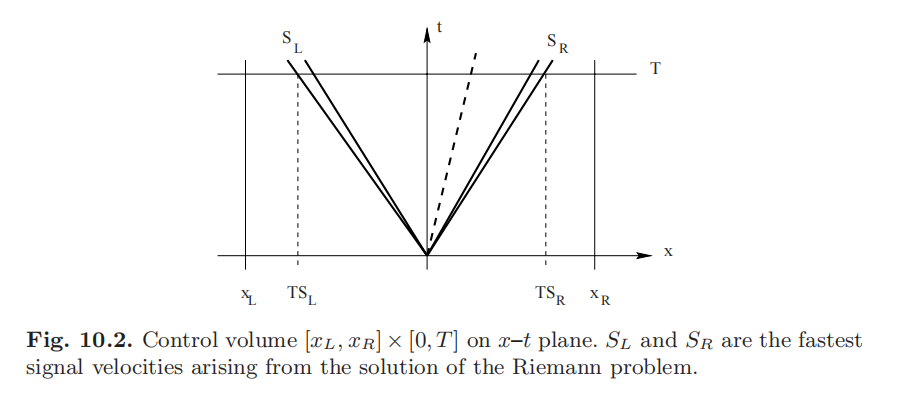
\includegraphics[width=0.7\linewidth]{fig/HLL.png}
    \caption{}
\end{figure}
考虑PDE在其上的积分形式:
\begin{equation}
    \displaystyle\int_{x_L}^{x_R}\mathbf U(x,t)\mathrm dx=\displaystyle\int_{x_L}^{x_R}\mathbf U(x,0)\mathrm dx+\int_{0}^T\mathbf F(\mathbf U(x_L,t))\mathrm dt-\int_0^T\mathbf F(\mathbf U(x_R,t))\mathrm dt
\end{equation}
后面三项都可以计算出来,从而得到
\begin{equation}
    \displaystyle\int_{x_L}^{x_R}\mathbf U(x,t)\mathrm dx=x_R\mathbf U_R-x_L\mathbf U_L+T(\mathbf F_L-\mathbf F_R)
\end{equation}
另一方面,我们有:
\begin{equation}
    \displaystyle\int_{x_L}^{x_R}\mathbf U(x,t)\mathrm dx=\int_{x_L}^{TS_L}+\int_{TS_L}^{TS_R}+\int_{TS_R}^{x_R}\mathbf U(x,t)\mathrm dx
\end{equation}
前一项和后一项都可以计算出来,从而得:
\begin{equation}
    \displaystyle\int_{x_L}^{x_R}\mathbf U(x,t)\mathrm dx=(TS_L-x_L)\mathbf U_L+\int_{TS_L}^{TS_R}\mathbf U(x,t)\mathrm dx+(x_R-TS_R)\mathbf U_R
\end{equation}
联立两式,得到:
\begin{equation}
    \displaystyle\int_{TS_L}^{TS_R}\mathbf U(x,t)\mathrm dx=T(S_R\mathbf U_R-S_L\mathbf U_L+\mathbf F_L-\mathbf F_R)
\end{equation}
从而单元平均值为:
\begin{equation}
    \displaystyle\frac{1}{T(S_R-S_L)}\int_{TS_L}^{TS_R}\mathbf U(x,t)\mathrm dx=\frac{S_R\mathbf U_R-S_L\mathbf U_L+\mathbf F_L-\mathbf F_R}{S_R-S_L}
\end{equation}
当 $T\to0^+$ ,我们得到 $\mathbf U^*$ 的近似状态:
\begin{equation}
    \mathbf U^{Hll}=\displaystyle\frac{S_R\mathbf U_R-S_L\mathbf U_L+\mathbf F_L-\mathbf F_R}{S_R-S_L}
\end{equation}
进一步,可以考虑如下的 $\bf U$ 的近似:
\begin{equation}
    \mathbf{\tilde{U}}\left( x,t \right) =\begin{cases}
        \mathbf{U}_L,x<S_Lt          \\
        \mathbf{U}^{Hll},S_Lt<x<S_Rt \\
        \mathbf{U}_R,x>S_Rt          \\
    \end{cases}
\end{equation}

设Star Region的Flux为 $\mathbf F^{Hll}$ ,则利用R-H跳跃条件,得到
\begin{equation}
    \mathbf{F}^{Hll}=\mathbf{F}_L+S_L\left( \mathbf{U}^{Hll}-\mathbf{U}_L \right)
\end{equation}
和
\begin{equation}
    \mathbf{F}^{Hll}=\mathbf{F}_R+S_R\left( \mathbf{U}^{Hll}-\mathbf{U}_R \right)
\end{equation}
这两个代进去算,结果是一样的,都可以解得
\begin{equation}
    \displaystyle \mathbf{F}^{Hll}=\frac{S_R\mathbf{F}_L-S_L\mathbf{F}_R+S_LS_R\left( \mathbf{U}_R-\mathbf{U}_L \right)}{S_R-S_L}
\end{equation}
从而,HLL Flux的定义为:
\begin{equation}
    \mathbf{F}_{i+1/2}^{Hll}=\begin{cases}
        \mathbf{F}_L,S_L\ge 0      \\
        \mathbf{F}^{Hll},S_L<0<S_R \\
        \mathbf{F}_R,S_R\le 0      \\
    \end{cases}
\end{equation}





\subsection{HLLC Flux}
HLLC Flux的近似更为精细,但计算也更复杂。假设除了两个激波外,还有一个波速为 $S_*$ 的接触波,满足
\begin{equation}
    S_L<S_*<S_R
\end{equation}
如图:
\begin{figure}[htp]
    \centering
    \label{fig:}
    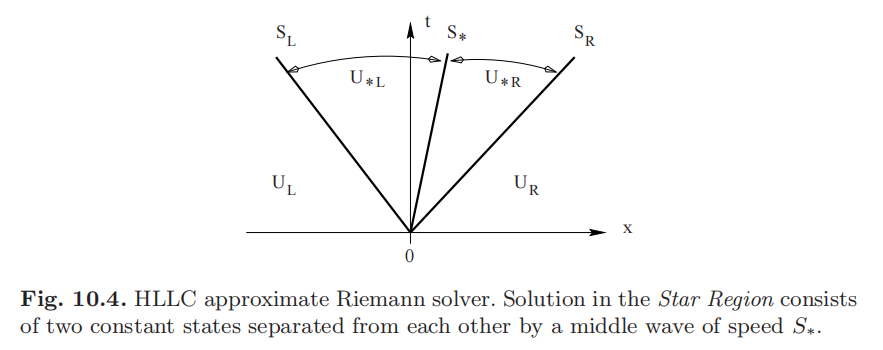
\includegraphics[width=0.7\linewidth]{fig/HLLC.png}
    \caption{}
\end{figure}


则Star Region中有两个未知状态: $\mathbf U_{*,L}$ 和 $\mathbf U_{*,R}$ 。仍然利用之前的控制体 $[x_L,x_R]\times[0,T]$ ,我们可以写
\begin{equation}
    \begin{aligned}
        \mathbf U_{*,L} & =\displaystyle\frac{1}{T(S_*-S_L)}\int_{TS_L}^{TS_*}\mathbf U(x,t)\mathrm dx \\
        \mathbf U_{*,R} & =\displaystyle\frac{1}{T(S_R-S_*)}\int_{TS_*}^{TS_R}\mathbf U(x,t)\mathrm dx
    \end{aligned}
\end{equation}
由于我们还有
\begin{equation}
    \mathbf U^{Hll}=\displaystyle\frac{1}{T(S_R-S_L)}\int_{TS_L}^{TS_R}\mathbf U(x,t)\mathrm dx
\end{equation}
从而得到
\begin{equation}
    \displaystyle \left( \frac{S_*-S_L}{S_R-S_L} \right) \mathbf{U}_{*,L}+\left( \frac{S_R-S_*}{S_R-S_L} \right) \mathbf{U}_{*,R}=\mathbf{U}^{Hll}
\end{equation}
注意这里新的接触波的加入并不影响 $\mathbf U^{Hll}$ 之前的推导,因此我们仍然有
\begin{equation}
    \mathbf U^{Hll}=\displaystyle\frac{S_R\mathbf U_R-S_L\mathbf U_L+\mathbf F_L-\mathbf F_R}{S_R-S_L}
\end{equation}
HLLC Flux的定义方式如下,与HLL Flux基本相同:
\begin{equation}
    \mathbf{\tilde{U}}=\left\{ \begin{array}{l} \mathbf{U}_L,x<S_Lt\\ \mathbf{U}_{*,L},S_Lt<x<S_*t\\ \mathbf{U}_{*,R},S_*t<x<S_Rt\\ \mathbf{U}_R,S_Rt<x\\ \end{array} \right.
\end{equation}
对应的Flux为
\begin{equation}
    \mathbf{F}_{i+1/2}^{Hllc}=\left\{ \begin{array}{l} \mathbf{F}_L,S_L>0\\ \mathbf{F}_{*,L},S_L<0<S_*\\ \mathbf{F}_{*,R},S_*<0<S_R\\ \mathbf{F}_R,S_R<0\\ \end{array} \right.
\end{equation}
现在我们需要决定四个未知状态 $\mathbf U_{*,L}$,\ $\mathbf U_{*,R}$,\ $\mathbf F_{*,L}$,\ $\mathbf F_{*,R}$ 。利用R-H跳跃条件,可以列出三个关系式:
\begin{equation}
    \begin{aligned}
        \mathbf{F}_{*,L}-\mathbf{F}_L     & =S_L\left( \mathbf{U}_{*,L}-\mathbf{U}_L \right)     \\
        \mathbf{F}_{*,R}-\mathbf{F}_{*,L} & =S_*\left( \mathbf{U}_{*,R}-\mathbf{U}_{*,L} \right) \\
        \mathbf{F}_R-\mathbf{F}_{*,R}     & =S_R\left( \mathbf{U}_R-\mathbf{U}_{*,R} \right)
    \end{aligned}
\end{equation}
现在我们考虑Euler方程在 x 分量上的Flux:
\begin{equation}
    \mathbf{F}\left( \mathbf{U} \right) =\left[ \begin{array}{l} \rho u\\ \rho u^2+p\\ \rho uv\\ \rho uw\\ u\left( E+p \right)\\ \end{array} \right]
\end{equation}
根据方程本身的性质,我们附加以下条件:

1. 压强和法向速度是连续的:
\begin{equation}
    p_{*,L}=p_{*,R}=:p_*
\end{equation}
\begin{equation}
    u_{*,L}=u_{*,R}=:u_*
\end{equation}
2. 其它两个速度在左、右分别等于左右的初值:
\begin{equation}
    v_{*,L}=v_L,\ v_{*,R}=v_R
\end{equation}
\begin{equation}
    w_{*,L}=w_L,\ w_{*,R}=w_R
\end{equation}
3. 接触波的速度
\begin{equation}
    S^*=u
\end{equation}
注意到一个重要的关系式
\begin{equation}
    \mathbf{F}\left( \mathbf{U} \right) =\left[ \begin{array}{l} \rho u\\ \rho u^2+p\\ \rho uv\\ \rho uw\\ u\left( E+p \right)\\ \end{array} \right] =u\left[ \begin{array}{l} \rho\\ \rho u\\ \rho v\\ \rho w\\ E\\ \end{array} \right] +p\left[ \begin{array}{l} 0\\ 1\\ 0\\ 0\\ u\\ \end{array} \right] =:u\mathbf{U}+p\mathbf{D}
\end{equation}
因此,我们可将两个激波上的跳跃条件重写为
\begin{equation}
    S_L\mathbf{U}_{*,L}-\mathbf{F}_{*,L}=S_L\mathbf{U}_L-\mathbf{F}_L
\end{equation}
\begin{equation}
    S_R\mathbf{U}_{*,R}-\mathbf{F}_{*,R}=S_R\mathbf{U}_R-\mathbf{F}_R
\end{equation}
考虑第一个式子的第一个分量:
\begin{equation}
    S_L\rho_{*,L}-\rho_{*,L}u_{*,L}                        = S_L\rho_L-\rho_Lu_L
\end{equation}
考虑第一个式子的第二个分量:
\begin{equation}
    \begin{aligned}
        S_L\rho_{*,L}u_{*,L}-u_{*,L}\rho_{*,L}u_{*,L}-p_{*,L} -p_{*,L} & = S_L\rho_L u_L - u_L\rho_Lu_L-p_L \\
        (S_L-u_{*,L})\rho_{*,L}u_{*,L}      -p_{*,L}                   & = (S_L-u_L)\rho_Lu_L-p_L
    \end{aligned}
\end{equation}
将上上式带入上式,得到:
\begin{equation}
    (S_L-u_L)\rho_Lu_{*,L}      -p_{*,L}  = (S_L-u_L)\rho_Lu_L-p_L
\end{equation}
从而:
\begin{equation}
    p_{*,L} =  p_L+\rho_L(S_L-u_L)(S_*-u_L)
\end{equation}
同理:
\begin{equation}
    p_{*,R}=p_R+\rho _R\left( S_R-u_R \right) \left( S_*-u_R \right)
\end{equation}
由于 $p_{*,L}=p_{*,R}$ ,联立上述两式即可解出接触波的波速 $S_*$ (注意它也等于法向的速度 $u$ )为:
\begin{equation}
    \displaystyle S_*=\frac{p_R-p_L+\rho _Lu_L\left( S_L-u_L \right) -\rho _Ru_R\left( S_R-u_R \right)}{\rho _L\left( S_L-u_L \right) -\rho _R\left( S_R-u_R \right)}
\end{equation}
并且 $S_L$,$S_R$ 是已知的,我们现在只需要利用R-H跳跃条件即可解出HLLC Flux。

利用 $\mathbf F(\mathbf U)=u\mathbf U+p\mathbf D$ ,我们可以将激波的跳跃条件重写为
\begin{equation}
    S_*\mathbf{U}_{*,K}+p_*\mathbf{D}_*=\mathbf{F}_K+S_K\mathbf{U}_{*,K}-S_K\mathbf{U}_K
\end{equation}
其中 $K=L,R$ ,因此
\begin{equation}
    \displaystyle \mathbf{U}_{*,K}=\frac{S_K\mathbf{U}_K-\mathbf{F}_K+p_*\mathbf{D}_*}{S_K-S_*}
\end{equation}
再用一次跳跃条件,即得到直接的表达式:
\begin{equation}
    \displaystyle \mathbf{F}_{*,K}=\frac{S_*\left( S_K\mathbf{U}_K-\mathbf{F}_K \right) +S_K\left( p_K+\rho _L\left( S_K-u_K \right) \left( S_*-u_K \right) \right) \mathbf{D}_*}{S_K-S_*}
\end{equation}

\subsection{波速估计}
\subsubsection{估计方法1}
% A positivity-preserving high-order weighted compact nonlinear scheme for compressible gas-liquid flows
% https://www.sciencedirect.com/science/article/abs/pii/S0021999121004642
\begin{equation}
    s_{L}=\min \left(\bar{u}-\bar{c}, u_{L}-c_{L}\right), \quad s_{R}=\max \left(\bar{u}+\bar{c}, u_{R}+c_{R}\right),
\end{equation}
其中
\begin{equation}
    \begin{aligned}
        \bar{u}     & =\frac{u_{L} \sqrt{\rho_{L}}+u_{R} \sqrt{\rho_{R}}}{\sqrt{\rho_{L}}+\sqrt{\rho_{R}}}                                                                                                                                            \\
        \bar{c}^{2} & =\frac{c_{L}^{2} \sqrt{\rho_{L}}+c_{R}^{2} \sqrt{\rho_{R}}}{\sqrt{\rho_{L}}+\sqrt{\rho_{R}}}+\frac{1}{2} \frac{\sqrt{\rho_{L}} \sqrt{\rho_{R}}}{\left(\sqrt{\rho_{L}}+\sqrt{\rho_{R}}\right)^{2}}\left(u_{R}-u_{L}\right)^{2} .
    \end{aligned}
\end{equation}
\subsubsection{估计方法2}
这里给出一种估计 $S_L,S_R$ 的方法\cite{numFlux2}:
\begin{equation}
    s_L=v_L-c_L q_L, \quad s^{*}=v^{*}, \quad s_R=v_R+c_R q_R,
\end{equation}
其中, for  $K=L,R$ ,
\begin{equation}
    q^{K}=\begin{cases}
        1                                                                            & \text { if } p^{*} \leqslant p^{K}, \\
        \left(1+\frac{\gamma+1}{2 \gamma}\left(p^{*} / p^{K}-1\right)\right)^{1 / 2} & \text { if } p^{*}>p^{K},
    \end{cases}
\end{equation}
其中
\begin{equation}
    p^{*}=\frac{1}{2}\left(p_L+p_R\right)-\frac{1}{2}\left(v_R-v_L\right) \bar{\rho} \bar{c}, \quad v^{*}=\frac{1}{2}\left(v_L+v_R\right)-\frac{p_R-p_L}{2 \bar{\rho} \bar{c}},
\end{equation}
其中
\begin{equation}
    \bar{\rho}=\frac{1}{2}\left(\rho_L+\rho_R\right), \quad \bar{c}=\frac{1}{2}\left(c_L+c_R\right) .
\end{equation}
\section{双曲型方程(hyperbolic equation)}
\begin{figure}[htp]
    \centering
    \label{fig:间断波}
    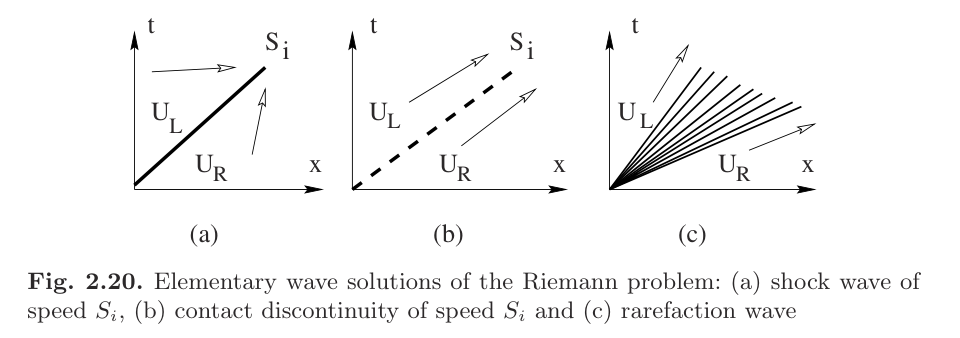
\includegraphics[width=0.7\linewidth]{fig/间断波.png}
    \caption{Elementary wave solutions of the Riemann problem: (a) shock wave of speed  $S_{i}$ , (b) contact discontinuity of speed  $S_{i}$  and (c) rarefaction wave}
\end{figure}

\subsection{激波(Shock Wave)}
For a shock wave the two constant states  $\mathbf{U}_{\mathrm{L}}$  and  $\mathbf{U}_{\mathrm{R}}$  are connected through a single jump discontinuity in a genuinely non-linear field  i  and the following conditions apply
the Rankine-Hugoniot conditions
\begin{equation}
    \mathbf{F}\left(\mathbf{U}_{\mathrm{R}}\right)-\mathbf{F}\left(\mathbf{U}_{\mathrm{L}}\right)=S_{i}\left(\mathbf{U}_{\mathrm{R}}-\mathbf{U}_{\mathrm{L}}\right) .
\end{equation}
the entropy condition
\begin{equation}
    \lambda_{i}\left(\mathbf{U}_{\mathrm{L}}\right)>S_{i}>\lambda_{i}\left(\mathbf{U}_{\mathrm{R}}\right)
\end{equation}
Fig. 2.20a depicts a shock wave of speed  $S_{i}$ . The characteristic  $\mathrm{d} x / \mathrm{d} t=\lambda_{i}$  on both sides of the wave run into the shock wave, which illustrates the compressive character of a shock.
\subsection{接触间断(Rarefaction Wave)}
For a contact wave the two data states  $\mathbf{U}_{\mathrm{L}}$  and  $\mathbf{U}_{\mathrm{R}}$  are connected through a single jump discontinuity of speed  $S_{i}$  in a linearly degenerate field  i  and the following conditions apply
the Rankine-Hugoniot conditions
\begin{equation}
    \mathbf{F}\left(\mathbf{U}_{\mathrm{R}}\right)-\mathbf{F}\left(\mathbf{U}_{\mathrm{L}}\right)=S_{i}\left(\mathbf{U}_{\mathrm{R}}-\mathbf{U}_{\mathrm{L}}\right)
\end{equation}
constancy of the Generalised Riemann Invariants across the wave
\begin{equation}
    \frac{\mathrm{d} w_{1}}{k_{1}^{(i)}}=\frac{\mathrm{d} w_{2}}{k_{2}^{(i)}}=\frac{\mathrm{d} w_{3}}{k_{3}^{(i)}}=\cdots=\frac{\mathrm{d} w_{m}}{k_{m}^{(i)}} .
\end{equation}
the parallel characteristic condition
\begin{equation}
    \lambda_{i}\left(\mathbf{U}_{\mathrm{L}}\right)=\lambda_{i}\left(\mathbf{U}_{\mathrm{R}}\right)=S_{i}
\end{equation}
Fig. 2.20b depicts a contact discontinuity. Characteristics on both sides of the wave run parallel to it.


\subsection{稀疏波(Rarefaction Wave)}
For a rarefaction wave the two data states  $\mathbf{U}_{\mathrm{L}}$  and  $\mathbf{U}_{\mathrm{R}}$  are connected through a smooth transition in a genuinely non-linear field  i  and the following conditions are met
constancy of the Generalised Riemann Invariants across the wave
\begin{equation}
    \frac{\mathrm{d} w_{1}}{k_{1}^{(i)}}=\frac{\mathrm{d} w_{2}}{k_{2}^{(i)}}=\frac{\mathrm{d} w_{3}}{k_{3}^{(i)}}=\cdots=\frac{\mathrm{d} w_{m}}{k_{m}^{(i)}} .
\end{equation}
divergence of characteristics
\begin{equation}
    \lambda_{i}\left(\mathbf{U}_{\mathrm{L}}\right)<\lambda_{i}\left(\mathbf{U}_{\mathrm{R}}\right)
\end{equation}
Fig. 2.20c depicts a rarefaction wave. Characteristics on the left and right of the wave diverge as do characteristics inside the wave.

\chapter{附录}
\section{模板}
\begin{table}[ht]
    \small
    \centering
    \begin{tabular}{|c|c|cccc|cccc|}
        \hline
                               &                 & \multicolumn{4}{c|}{DG   with MRWENO limiter} & \multicolumn{4}{c|}{DG   with WENO-JS limiter}                                                                                                                                                                 \\ \hline
                               & $N\times N$     & \multicolumn{1}{c|}{$L_1$ error}              & \multicolumn{1}{c|}{Order}                     & \multicolumn{1}{c|}{$L_\infty$ error} & Order & \multicolumn{1}{c|}{$L_1$ error} & \multicolumn{1}{c|}{Order} & \multicolumn{1}{c|}{$L_\infty$ error} & Order \\ \hline
        \multirow{6}{*}{$P^1$} & $50\times 50$   & \multicolumn{1}{c|}{8.74E-05}                 & \multicolumn{1}{c|}{}                          & \multicolumn{1}{c|}{1.38E-04}         &       & \multicolumn{1}{c|}{1.97E-04}    & \multicolumn{1}{c|}{}      & \multicolumn{1}{c|}{8.99E-04}         &       \\ \cline{2-10}
                               & $60\times 60$   & \multicolumn{1}{c|}{5.77E-05}                 & \multicolumn{1}{c|}{2.28}                      & \multicolumn{1}{c|}{9.07E-05}         & 2.30  & \multicolumn{1}{c|}{1.01E-04}    & \multicolumn{1}{c|}{3.68}  & \multicolumn{1}{c|}{5.51E-04}         & 2.68  \\ \cline{2-10}
                               & $70\times 70$   & \multicolumn{1}{c|}{4.09E-05}                 & \multicolumn{1}{c|}{2.22}                      & \multicolumn{1}{c|}{6.41E-05}         & 2.25  & \multicolumn{1}{c|}{6.18E-05}    & \multicolumn{1}{c|}{3.16}  & \multicolumn{1}{c|}{2.89E-04}         & 4.18  \\ \cline{2-10}
                               & $80\times 80$   & \multicolumn{1}{c|}{3.08E-05}                 & \multicolumn{1}{c|}{2.14}                      & \multicolumn{1}{c|}{4.83E-05}         & 2.11  & \multicolumn{1}{c|}{4.44E-05}    & \multicolumn{1}{c|}{2.48}  & \multicolumn{1}{c|}{1.85E-04}         & 3.34  \\ \cline{2-10}
                               & $90\times 90$   & \multicolumn{1}{c|}{2.40E-05}                 & \multicolumn{1}{c|}{2.11}                      & \multicolumn{1}{c|}{3.77E-05}         & 2.10  & \multicolumn{1}{c|}{3.16E-05}    & \multicolumn{1}{c|}{2.89}  & \multicolumn{1}{c|}{1.27E-04}         & 3.22  \\ \cline{2-10}
                               & $100\times 100$ & \multicolumn{1}{c|}{1.93E-05}                 & \multicolumn{1}{c|}{2.09}                      & \multicolumn{1}{c|}{3.02E-05}         & 2.09  & \multicolumn{1}{c|}{2.47E-05}    & \multicolumn{1}{c|}{2.33}  & \multicolumn{1}{c|}{8.66E-05}         & 3.62  \\ \hline
        \multirow{6}{*}{$P^2$} & $50\times 50$   & \multicolumn{1}{c|}{3.60E-06}                 & \multicolumn{1}{c|}{}                          & \multicolumn{1}{c|}{5.14E-06}         &       & \multicolumn{1}{c|}{3.59E-06}    & \multicolumn{1}{c|}{}      & \multicolumn{1}{c|}{5.14E-06}         &       \\ \cline{2-10}
                               & $60\times 60$   & \multicolumn{1}{c|}{2.08E-06}                 & \multicolumn{1}{c|}{3.02}                      & \multicolumn{1}{c|}{3.01E-06}         & 2.93  & \multicolumn{1}{c|}{2.07E-06}    & \multicolumn{1}{c|}{3.01}  & \multicolumn{1}{c|}{3.01E-06}         & 2.93  \\ \cline{2-10}
                               & $70\times 70$   & \multicolumn{1}{c|}{1.30E-06}                 & \multicolumn{1}{c|}{3.03}                      & \multicolumn{1}{c|}{1.91E-06}         & 2.95  & \multicolumn{1}{c|}{1.30E-06}    & \multicolumn{1}{c|}{3.02}  & \multicolumn{1}{c|}{1.91E-06}         & 2.95  \\ \cline{2-10}
                               & $80\times 80$   & \multicolumn{1}{c|}{8.69E-07}                 & \multicolumn{1}{c|}{3.03}                      & \multicolumn{1}{c|}{1.29E-06}         & 2.96  & \multicolumn{1}{c|}{8.68E-07}    & \multicolumn{1}{c|}{3.03}  & \multicolumn{1}{c|}{1.29E-06}         & 2.96  \\ \cline{2-10}
                               & $90\times 90$   & \multicolumn{1}{c|}{6.08E-07}                 & \multicolumn{1}{c|}{3.03}                      & \multicolumn{1}{c|}{9.08E-07}         & 2.97  & \multicolumn{1}{c|}{6.08E-07}    & \multicolumn{1}{c|}{3.02}  & \multicolumn{1}{c|}{9.08E-07}         & 2.97  \\ \cline{2-10}
                               & $100\times 100$ & \multicolumn{1}{c|}{4.42E-07}                 & \multicolumn{1}{c|}{3.03}                      & \multicolumn{1}{c|}{6.64E-07}         & 2.97  & \multicolumn{1}{c|}{4.42E-07}    & \multicolumn{1}{c|}{3.03}  & \multicolumn{1}{c|}{6.64E-07}         & 2.97  \\ \hline
    \end{tabular}
\end{table}

\section{WENO3与WENO5参数求解过程}
WENO5 重构多项式:
\begin{equation}
    \begin{aligned}
        P_0(x) & = \frac{1}{2} \left(u_{i}^{(0)} - 2 u_{i-1}^{(0)} + u_{i-2}^{(0)}\right)x^2 + \frac{1}{2} \left(3  u_{i}^{(0)} - 4 u_{i-1}^{(0)} + u_{i-2}^{(0)}\right)  x + \frac{23}{24}u_{i}^{(0)} +\frac{1}{12} u_{i-1}^{(0)} -\frac{1}{24} u_{i-2}^{(0)}        \\
        P_1(x) & = \frac{1}{2} \left(u_{i+1}^{(0)} - 2  u_{i}^{(0)} + u_{i-1}^{(0)}\right)x^2 + \frac{1}{2}  \left(u_{i+1}^{(0)} - u_{i-1}^{(0)}\right)  x -\frac{1}{24}  u_{i+1}^{(0)} + \frac{13}{12}  u_{i}^{(0)} -\frac{1}{24}  u_{i-1}^{(0)}                     \\
        P_2(x) & = \frac{1}{2}  \left(u_{i}^{(0)} - 2  u_{i+1}^{(0)} + u_{i+2}^{(0)}\right)x^2 + \frac{1}{2}\left(4  u_{i+1}^{(0)} - u_{i+2}^{(0)} - 3  u_{i}^{(0)}\right)  x + \frac{1}{12}  u_{i+1}^{(0)} -\frac{1}{24}  u_{i+2}^{(0)} + \frac{23}{24}  u_{i}^{(0)}
    \end{aligned}
\end{equation}
满足:
\begin{equation}
    \begin{aligned}
        \int_{-5/2}^{-3/2} P_0(x)\dd x = u_{i-2}^{(0)},\quad \int_{-3/2}^{-1/2} P_0(x)\dd x = u_{i-1}^{(0)},\quad \int_{-1/2}^{1/2} P_0(x)\dd x = u_{i}^{(0)} \\
        \int_{-3/2}^{-1/2} P_1(x)\dd x = u_{i-1}^{(0)},\quad \int_{-1/2}^{1/2} P_1(x)\dd x = u_{i}^{(0)},\quad \int_{1/2}^{3/2} P_1(x)\dd x = u_{i+1}^{(0)}   \\
        \int_{-1/2}^{1/2} P_2(x)\dd x = u_{i}^{(0)},\quad \int_{1/2}^{3/2} P_2(x)\dd x = u_{i+1}^{(0)},\quad \int_{3/2}^{5/2} P_2(x)\dd x = u_{i+2}^{(0)}     \\
    \end{aligned}
\end{equation}






\section{编程小技巧}
\subsection{程序加速}
\begin{itemize}
    \item 使用linux系统似乎会加快计算速度。
    \item 使用并行算法可以显著提升速度。
    \item 使用 c++, Fortran 等编译型语言放弃 MATLAB等解释型语言
    \item 使用自适应网络。
    \item 使用合适的CFL数与合适的高斯积分点。
    \item 在初始化的时候储存基函数 $\varphi(x)$ 在高斯点处的值,从而省去每次计算 $\varphi(x_0)$ 。
\end{itemize}
% https://www.zhihu.com/question/68169365/answer/524351247
% https://zhuanlan.zhihu.com/p/533958396 储存高斯点
\subsection{检查程序错误}
\begin{itemize}
    \item 只完成初始化,不做时间推进,然后测试精度是否满足预期。这样可以检查初始化与精度计算是否有误。
    \item 左右特征向量矩阵相乘,检验是否得到单位矩阵。这样可以检查特征向量矩阵是否写错。
    \item 在测试二维程序的时候,将一个一维问题延拓成二维问题,并把计算结果与一维问题的情况做对比。
    \item 在测试二维程序的时候,先找一个对称的问题,检查计算结果是否对称。
    \item 先使用 L-F , P1 这样简单的设置,再尝试复杂的设置。
    \item 先计算结构化网络,再计算非结构化网络。
          % https://en.wikipedia.org/wiki/Mesh_generation
    \item 保极值限制器中 $\epsilon$ 不宜太小,参考值:1e-8~1e-13
    \item 太少的网格数量也可能会导致程序出错
\end{itemize}

\section{边界条件}
\subsection{周期性边界条件}
\subsection{常数边界条件}
\subsection{反射边界条件}
\subsection{滑移边界条件}


\section{数学符号}
\subsection{散度}
\href{https://zh.wikipedia.org/zh-hans/%E6%95%A3%E5%BA%A6}{维基百科:散度} 
在三维直角坐标系  $x y z$  中,设向量场  $\boldsymbol{A}$  的表示为
$\boldsymbol{A}(x, y, z)=A_{x}(x, y, z) \boldsymbol{i}+A_{y}(x, y, z) \boldsymbol{j}+A_{z}(x, y, z) \boldsymbol{k}$ 其中的  $\boldsymbol{i}, \boldsymbol{j}, \boldsymbol{k} $ 分别是  $x$  轴、  $y$  轴、  $z$  轴方向上的单位向量,场的分量  $A_{x}, A_{y}, A_{z}$  具有一阶连续偏导数,那么向量场  $\boldsymbol{A}$  的散度就是:
\begin{equation}
    \operatorname{div} \boldsymbol{A}=\div \boldsymbol{A}=\dfrac{\partial A_{x}}{\partial x}+\dfrac{\partial A_{y}}{\partial y}+\dfrac{\partial A_{z}}{\partial z}
\end{equation}
\subsection{拉普拉斯算子}
\href{https://zh.wikipedia.org/zh-hans/%E6%8B%89%E6%99%AE%E6%8B%89%E6%96%AF%E7%AE%97%E5%AD%90}{text}
\subsection{维基百科:拉普拉斯算子}
$\nabla f$在三维直角坐标系中表示为
\begin{equation}
    {\displaystyle \nabla f={\begin{pmatrix}{\dfrac {\partial f}{\partial x}},{\dfrac {\partial f}{\partial y}},{\dfrac {\partial f}{\partial z}}\end{pmatrix}}={\dfrac {\partial f}{\partial x}}\mathbf {i} +{\dfrac {\partial f}{\partial y}}\mathbf {j} +{\dfrac {\partial f}{\partial z}}\mathbf {k} }
\end{equation}
$i, j, k $为标准的单位向量,分别指向 $x, y$ 跟 $z$ 坐标的方向.
\subsection{范数}
范数(norm)是一个函数,它将一个向量映射到非负实数.在机器学习和优化中,范数是一种衡量向量大小或长度的方式.

L1, L2和L无穷范数是线性代数中的三种不同的向量范数(或向量长度度量),它们在数学和数据科学领域中经常使用.

L1范数:L1范数也称为曼哈顿距离,它是一个向量中每个元素的绝对值之和.对于一个$n$维向量$x = (x1, x2, ..., xn)$,其$L1$范数定义如下:
\begin{equation}
    ||x||_1 = |x_1| + |x_2| + \cdots + |x_n|
\end{equation}

L2范数:L2范数也称为欧几里得距离,它是向量中每个元素平方和的平方根.对于一个$n$维向量$x = (x_1, x_2,\cdots, x_n)$,其L2范数定义如下:
\begin{equation}
    ||x||_2 = \sqrt{(x_1^2 + x_2^2 + ... + x_n^2)}
\end{equation}
$L_\infty$范数:$L_\infty$ 范数也称为最大值范数,它是向量中所有元素的绝对值中最大的值.对于一个n维向量$x = (x_1, x_2,\cdots, x_n)$,其$L_\infty$定义如下:
\begin{equation}
    ||x||_\infty = \max(|x_1|, |x_2|,\cdots, |x_n|)
\end{equation}
这些向量范数在机器学习和优化算法中经常使用,例如L1和L2正则化(用于缩小模型参数),L1和L2距离度量(用于计算相似性或距离),以及L1和L2约束(用于限制变量的取值范围).
\subsection{张量积}


\section{定义}
% https://en.wikipedia.org/wiki/Big_O_notation
\begin{definition}
    标准的巴赫曼-朗道符号(Bachmann-Landau notation) 如下:

    \begin{itemize}
        \item $g(\Delta x)=\mathrm{O}\left(\Delta x^{n}\right)$  意为: 存在常数 $C>0$,使得当 $\Delta x \rightarrow 0$时,$|g(\Delta x)| \leq C \Delta x^{n}$
        \item $g(\Delta x)=\Omega\left(\Delta x^{n}\right)$ 意为:  存在常数 $C>0$,使得当 $\Delta x \rightarrow 0$时,$|g(\Delta x)| \geq C \Delta x^{n}$
        \item $g(\Delta x)=\Theta\left(\Delta x^{n}\right)$  意为: 当 $\Delta x \rightarrow 0$ 时,$g(\Delta x)=\mathrm{O}\left(\Delta x^{n}\right)$  and  $g(\Delta x)=\Omega\left(\Delta x^{n}\right)$
    \end{itemize}

    请注意,根据这个定义,$g=\mathrm{O}(1)$ 并不意味着 $g$ 是一个常数; 相反,它意味着常数是 $g$ 的上限,即 $\Delta x \rightarrow 0$,或者换句话说,$g$ 不会随着 $\Delta x$ 渐近增长. 例如,此表示法中的 $\Delta x^{2 / 3}=\mathrm{O}(1)$.
\end{definition}
\begin{definition}
    如果$f\left(x_{c}\right)=f^{\prime}\left(x_{c}\right)=\ldots=f^{\left(n_{\mathrm{cp}}\right) }\left(x_{c}\right)=0$ 但 $f^{\left(n_{\mathrm{cp}}+1\right)}\left(x_{c}\right) \neq 0$,那么 $x_{c}$ 被认为是 $f(x)$ 的阶 $n_{\mathrm{cp}}$ 的临界点(critical point)。 如果 $f^{\prime}\left(x_{c}\right) \neq 0$,则 $x_{c}$ 被定义为 $f(x)$ 的 0 阶临界点。
\end{definition}
\begin{definition}
    \cite{WENO-Z-2016}
    If the smoothness indicator measures the smoothness of the whole  $R$  points stencil  $\mathcal{S}_{i+\frac{1}{2}}$ , it is called a global smoothness indicator; it is said to be a local smoothness indicator if it only acts in an  r  points substencil  $\mathcal{S}_{i+\frac{1}{2}}^{k} \subset \mathcal{S}_{i+\frac{1}{2}}$ .
\end{definition}
\begin{definition}
    \cite{WENO-Z-2016}
    simple critical points i.e.,  $x$  such that  $f^{\prime}(x)=0$  but  $f^{\prime \prime}(x) \neq 0$
\end{definition}
\begin{definition}
    \cite{WENO-Z-2016}
    flatter critical points (where$f^{\prime}(x)=f^{\prime \prime}(x)=0$)
\end{definition}
% \begin{definition}
%     $\theta(\psi(\Delta x))$  will denote the order of  $\psi$  (as a function of  $\Delta x$  ), that is, the power of  $\Delta x$  in the leading term of the asymptotic expansion of  $\psi(\Delta x)$ ,
%     \begin{equation}
%         \theta(\psi)=n \Longleftrightarrow \psi(\Delta x)=\Theta\left(\Delta x^{n}\right)
%     \end{equation}

%     $\theta_{0}(\psi(\Delta x)) $ will denote the order of  $\psi$  in the special case where the stencil is free of critical points.
% \end{definition}

\section{控制方程}
\subsection{一维方程}
\subsubsection{欧拉方程}
\paragraph{方程形式}
\begin{equation}
    \mathbf{U}=\left[\begin{array}{l}
            u_{1} \\
            u_{2} \\
            u_{3}
        \end{array}\right] \equiv\left[\begin{array}{c}
            \rho   \\
            \rho u \\
            E
        \end{array}\right], \quad \mathbf{F}=\left[\begin{array}{c}
            f_{1} \\
            f_{2} \\
            f_{3}
        \end{array}\right] \equiv\left[\begin{array}{c}
            \rho u       \\
            \rho u^{2}+p \\
            u(E+p)
        \end{array}\right]
\end{equation}
或
\begin{equation}
    \mathbf{F}(\mathbf{U})=\left[\begin{array}{l}
            f_{1} \\
            f_{2} \\
            f_{3}
        \end{array}\right] \equiv\left[\begin{array}{c}
            u_{2}                                                            \\
            \dfrac{1}{2}(3-\gamma) \dfrac{u_{2}^{2}}{u_{1}}+(\gamma-1) u_{3} \\
            \gamma \dfrac{u_{2}}{u_{1}} u_{3}-\dfrac{1}{2}(\gamma-1) \dfrac{u_{2}^{3}}{u_{1}^{2}}
        \end{array}\right]
\end{equation}
这里 $\rho$ 为密度,$p$为压力,$u$为粒子速度,$E$ 为每单位体积的总能量.
\begin{equation}
    E=\dfrac{1}{2}\rho u^{2}+\frac{p}{\gamma-1}
\end{equation}

对于空气,一般可取 $\gamma=1.4$.声速 $a$ 的表达式为:
\begin{equation}
    a=\sqrt{\left(p / \rho^{2}-e_{\rho}\right) / e_{p}}=\sqrt{\dfrac{\gamma p}{\rho}}
\end{equation}

\paragraph{特征分析}
Jacobian 矩阵为:
\begin{equation}
    \mathbf{A}(\mathbf{U})=\dfrac{\partial \mathbf{F}}{\partial \mathbf{U}}=\left[\begin{array}{l}
            \partial f_{1} / \partial u_{1} \partial f_{1} / \partial u_{2} \partial f_{1} / \partial u_{3} \\
            \partial f_{2} / \partial u_{1} \partial f_{2} / \partial u_{2} \partial f_{2} / \partial u_{3} \\
            \partial f_{3} / \partial u_{1} \partial f_{3} / \partial u_{2} \partial f_{3} / \partial u_{3}
        \end{array}\right]
\end{equation}

\begin{equation}
    \mathbf{A}(\mathbf{U})=\begin{bmatrix}
        0                                                                                      & 1                                                                                       & 0                                       \\
        -\dfrac{1}{2}(\gamma-3)\left(\dfrac{u_{2}}{u_{1}}\right)^{2}                           & (3-\gamma)\left(\dfrac{u_{2}}{u_{1}}\right)                                             & \gamma-1                                \\
        -\dfrac{\gamma u_{2} u_{3}}{u_{1}^{2}}+(\gamma-1)\left(\dfrac{u_{2}}{u_{1}}\right)^{3} & \dfrac{\gamma u_{3}}{u_{1}}-\dfrac{3}{2}(\gamma-1)\left(\dfrac{u_{2}}{u_{1}}\right)^{2} & \gamma\left(\dfrac{u_{2}}{u_{1}}\right)
    \end{bmatrix}
\end{equation}
\begin{equation}
    \begin{bmatrix}
        0                                          & 1                                                   & 0          \\
        -\dfrac{1}{2}(3-\gamma) u^{2}              & (3-\gamma) u                                        & (\gamma-1) \\
        -\gamma \dfrac{E u}{\rho}+(\gamma-1) u^{3} & \gamma \dfrac{E}{\rho}-\dfrac{3}{2}(\gamma-1) u^{2} & \gamma u
    \end{bmatrix}
\end{equation}

$\mathbf{A}(\mathbf{U})$ 的特征值为:
\begin{equation}
    \lambda_{1}=u-a, \lambda_{2}=u, \lambda_{3}=u+a
\end{equation}
左右特征向量为\cite{RN95}:
\begin{equation}
    L_{j}(u)=\left(\begin{array}{ccc}
            \dfrac{B_{2}+\mu / c}{2} & -\dfrac{B_{1} \mu+1 / c}{2} & \dfrac{B_{1}}{2} \\
            1-B_{2}                  & B_{1} \mu                   & -B_{1}           \\
            \dfrac{B_{2}-\mu / c}{2} & -\dfrac{B_{1} \mu-1 / c}{2} & \dfrac{B_{1}}{2}
        \end{array}\right)
\end{equation}
\begin{equation}
    R_{j}(u)=\left(\begin{array}{ccc}
            1       & 1           & 1       \\
            \mu-c   & \mu         & \mu+c   \\
            H-c \mu & \mu^{2} / 2 & H+c \mu
        \end{array}\right)
\end{equation}
$\text { where } c=\sqrt{\gamma p / \rho}, B_{1}=(\gamma-1) / c^{2}, B_{2}=B_{1} \mu^{2} / 2 \text { and } H=(E+p) / \rho \text {. }$
对应的右特征向量为:
\begin{equation}
    \mathbf{K}^{(1)}=\left[\begin{array}{c}
            1   \\
            u-a \\
            H-u a
        \end{array}\right], \mathbf{K}^{(2)}=\left[\begin{array}{c}
            1 \\
            u \\
            \dfrac{1}{2} u^{2}
        \end{array}\right], \mathbf{K}^{(3)}=\left[\begin{array}{c}
            1   \\
            u+a \\
            H+u a
        \end{array}\right]
\end{equation}
其中 $H$ 为总比焓(total specific enthalpy),$h$ 为比焓(specific enthalpy).
\begin{equation}
    H=(E+p) / \rho \equiv \dfrac{1}{2} u^{2}+h, \quad h=e+p / \rho
\end{equation}
\paragraph{算例}
\begin{example}[Linear Equation]
    We solve the linear equation\cite{RN56}:
    \begin{equation}
        \begin{aligned}
            u_{t}+u_{x} & =0 \quad-1<x<1,                    \\
            u(x, 0)     & =u_{0}(x) \quad \text { periodic }
        \end{aligned}
    \end{equation}
    其中:
    \begin{equation}
        \begin{aligned}
            u_{0}(x)        & =\begin{cases}
                                   \frac{1}{6}(G(x, \beta, z-\delta)+G(x, \beta, z+\delta)+4 G(x, \beta, z))    & -0.8 \leq x \leq-0.6 \\
                                   1                                                                            & -0.4 \leq x \leq-0.2 \\
                                   1-|10(x-0.1)|                                                                & 0 \leq x \leq 0.2    \\
                                   \frac{1}{6}(F(x, \alpha, a-\delta)+F(x, \alpha, a+\delta)+4 F(x, \alpha, a)) & 0.4 \leq x \leq 0.6  \\
                                   0                                                                            & \text { otherwise }
                               \end{cases} \\
            G(x, \beta, z)  & =e^{-\beta(x-z)^{2}}                                                                                 \\
            F(x, \alpha, a) & =\sqrt{\max \left(1-\alpha^{2}(x-a)^{2}, 0\right)}
        \end{aligned}
    \end{equation}
    常数取为$a=0.5, z=-0.7, \delta=0.005, \alpha=10$ 和 $\beta=\frac{\log 2}{36 \delta^{2}}$。该解包含了一个平滑但狭窄的高斯函数组合、一个方波、一个尖锐的三角波和一个半椭圆。

    结束时间为 $t=8$, 网格数量为200.
\end{example}
\begin{example}
    \cite{RN204}
    \begin{equation}
        u_0(x) = e^{-300*(x-x_c)^2},x_c=0.5
    \end{equation}
    $x\in[0,1]$ 周期边界条件,$t_end=1$

\end{example}
\begin{example}[Sod's shock-tube problem\cite{RN204}]
    \begin{equation}
        \begin{aligned}
            (\rho, u, p) & =(1,0,1)       & \text { 当 }0\leqslant x \leq 0.5,      \\
            (\rho, u, p) & =(0.125,0,0.1) & \text { 当 }0.5\leqslant x\leqslant 1 .
        \end{aligned}
    \end{equation}
    $t=0.2$
\end{example}
\begin{example}[interacting blast waves problem\cite{RN204}]
    \begin{equation}
        (\rho,u,p)=
        \begin{cases}
            (1,0,1000), if 0\leqslant x<0.1      \\
            (1,0,0.01), if 0.1 \leqslant x < 0.9 \\
            (1,0,100),if 0.9\leqslant x \leqslant 1
        \end{cases}
    \end{equation}

\end{example}
\begin{example}[Shu Osher 问题\cite{RN109}]
    \begin{equation}
        \begin{aligned}
            (\rho, v, p) & =(3.857143,2.629369,10.333333)   & \text { 当 } x \leq-4, \\
            (\rho, v, p) & =(1+\varepsilon \sin (5 x), 0,1) & \text { 当 } x>-4 .
        \end{aligned}
    \end{equation}
    选取 $\epsilon = 0.2$,计算区域为 $[-5,5]$,两端边界条件按初值条件给定后保持不变,求解至时间 $T=1.8$.
    \begin{figure}[htp]
        \centering
        \label{fig:shu_Osher}
        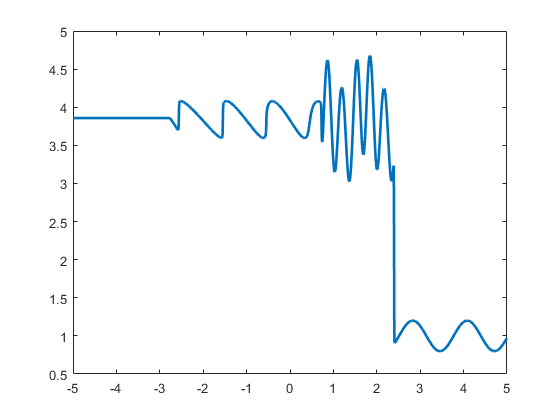
\includegraphics[width=0.7\linewidth]{fig/Shu_Osher.png}
        \caption{$N=2000,P2,WENO-JS,M=50$}
    \end{figure}

\end{example}

\subsection{二维方程}
\subsubsection{欧拉方程}
\paragraph{方程形式}
\begin{equation}
    \mathbf{U}_{t}+\mathbf{F}(\mathbf{U})_{x}+\mathbf{G}(\mathbf{U})_{y}=\mathbf{0}
\end{equation}
其中
\begin{equation}
    \mathbf{U}=\left[\begin{array}{c}
            \rho   \\
            \rho u \\
            \rho v \\
            E
        \end{array}\right], \quad \mathbf{F}=\left[\begin{array}{c}
            \rho u       \\
            \rho u^{2}+p \\
            \rho u v     \\
            u(E+p)
        \end{array}\right], \quad \mathbf{G}=\left[\begin{array}{c}
            \rho v       \\
            \rho u v     \\
            \rho v^{2}+p \\
            v(E+p)
        \end{array}\right]
\end{equation}
其中
\begin{equation}
    E=\dfrac{p}{\gamma-1}+\dfrac{1}{2} \rho\left(u^{2}+v^{2}\right)
\end{equation}
同时
\begin{equation}
    F = \begin{bmatrix}
        u_2                                                                          \\
        \dfrac{u_2^2}{u_1}+(\gamma-1)u_4+\dfrac{1-\gamma}{2}\dfrac{u_2^2+u_3^2}{u_1} \\
        \dfrac{u_2u_3}{u_1}                                                          \\
        \dfrac{u_2}{u_1}\left(\gamma u_4+\dfrac{1-\gamma}{2}\dfrac{u_2^2+u_3^2}{u_1}\right)
    \end{bmatrix}
    ,\quad G=\begin{bmatrix}
        u_3                                                                          \\
        \dfrac{u_2u_3}{u_1}                                                          \\
        \dfrac{u_3^2}{u_1}+(\gamma-1)u_4+\dfrac{1-\gamma}{2}\dfrac{u_2^2+u_3^2}{u_1} \\
        \dfrac{u_3}{u_1}\left(\gamma u_4+\dfrac{1-\gamma}{2}\dfrac{u_2^2+u_3^2}{u_1}\right)
    \end{bmatrix}
\end{equation}

\paragraph{特征分析}
特征值为
\begin{equation}
    \lambda_{1}=u-a, \quad \lambda_{2}=\lambda_{3}=u, \quad \lambda_{4}=u+a
\end{equation}

\begin{equation}
    \begin{bmatrix}
        0                                                                                                & 1                                                                                                   & 0                                         & 0                           \\
        \dfrac{\gamma (u_{2}-3)^{2}+(\gamma-1) u_{3}^{2}}{2 u_{1}^{2}}                                   & -(\gamma-3)\dfrac{u_{2}}{u_{1}}                                                                     & -(\gamma-1)\dfrac{u_{3}}{u_{1}}           & \gamma-1                    \\
        -\dfrac{u_{2} u_{3}}{u_{1}^{2}}                                                                  & \dfrac{u_{3}}{u_{1}}                                                                                & \dfrac{u_{2}}{u_{1}}                      & 0                           \\
        \dfrac{u_{2}}{u_1}\dfrac{\left((\gamma-1)(u_{2}^{2}+u_3^2)-\gamma u_{1} u_{4}\right)}{u_{1}^{2}} & \dfrac{3 u_{2}^{2}-\gamma u_{3}^{2}-3 \gamma u_{2}^{2}+u_{3}^{2}+2 \gamma u_{1} u_{4}}{2 u_{1}^{2}} & -\dfrac{u_{2} u_{3}(\gamma-1)}{u_{1}^{2}} & \dfrac{\gamma u_{2}}{u_{1}}
    \end{bmatrix}
\end{equation}
\begin{equation}
    \begin{bmatrix}
        0                                                                                             & 0                                                        & 1                                                                                       & 0                           \\
        -\dfrac{u_2 \,u_3 }{{u_1 }^2 }                                                                & \dfrac{u_3 }{u_1 }                                       & \dfrac{u_2 }{u_1 }                                                                      & 0                           \\
        \dfrac{\gamma \,{u_2 }^2 +\gamma \,{u_3 }^2 -{u_2 }^2 -3\,{u_3 }^2 }{2\,{u_1 }^2 }            & -\dfrac{u_2 \,{\left(\gamma -1\right)}}{u_1 }            & -\dfrac{u_3 \,{\left(\gamma -3\right)}}{u_1 }                                           & \gamma -1                   \\
        \dfrac{u_3}{u_1}\dfrac{{\left((\gamma-1)(u_2^2+u_3^2)-\gamma \,u_1 \,u_4 \right)}}{{u_1 }^2 } & -{\left(\gamma -1\right)}\dfrac{u_2 \,u_3 \,}{{u_1 }^2 } & \dfrac{(1-\gamma){u_2 }^2 +3(1-\gamma)\,{u_3 }^2 +2\,\gamma \,u_1 \,u_4 }{2\,{u_1 }^2 } & \dfrac{\gamma \,u_3 }{u_1 }
    \end{bmatrix}
\end{equation}

\begin{equation}
    F_U=\begin{bmatrix}
        0                                                     & 1                  & 0               & 0        \\
        -u^{2}+\dfrac{1}{2}(\gamma-1) \mathbf{V}^{2}          & (3-\gamma) u       & -(\gamma-1) v   & \gamma-1 \\
        -u v                                                  & v                  & u               & 0        \\
        u\left[\dfrac{1}{2}(\gamma-1) \mathbf{V}^{2}-H\right] & H-(\gamma-1) u^{2} & -(\gamma-1) u v & \gamma u
    \end{bmatrix} .
\end{equation}
其中 $\mathbf{V}^2=v^2+u^2$,

左右特征向量为\cite{RN95}:
\begin{equation}
    L_{i j}^{x}(u)=\begin{bmatrix}
        \dfrac{B_{2}+\mu / c}{2} & -\dfrac{B_{1} \mu+1 / c}{2} & -\dfrac{B_{1} v}{2} & \dfrac{B_{1}}{2} \\
        v                        & 0                           & -1                  & 0                \\
        1-B_{2}                  & B_{1} \mu                   & B_{1} v             & -B_{1}           \\
        \dfrac{B_{2}-\mu / c}{2} & -\dfrac{B_{1} \mu-1 / c}{2} & -\dfrac{B_{1} v}{2} & \dfrac{B_{1}}{2}
    \end{bmatrix},\quad
    R_{i j}^{x}(u)=\begin{bmatrix}
        1       & 0  & 1                        & 1       \\
        \mu-c   & 0  & \mu                      & \mu+c   \\
        v       & -1 & v                        & v       \\
        H-c \mu & -v & \dfrac{\mu^{2}+v^{2}}{2} & H+c \mu
    \end{bmatrix}
\end{equation}

\begin{equation}
    L_{i j}^{y}(u)=\begin{bmatrix}
        \dfrac{B_{2}+v / c}{2} & -\dfrac{B_{1} \mu}{2} & -\dfrac{B_{1} v+1 / c}{2} & \dfrac{B_{1}}{2} \\
        -\mu                   & 1                     & 0                         & 0                \\
        1-B_{2}                & B_{1} \mu             & B_{1} v                   & -B_{1}           \\
        \dfrac{B_{2}-v / c}{2} & -\dfrac{B_{1} \mu}{2} & -\dfrac{B_{1} v-1 / c}{2} & \dfrac{B_{1}}{2}
    \end{bmatrix},\quad
    R_{i j}^{y}(u)=\begin{bmatrix}
        1     & 0   & 1                        & 1     \\
        \mu   & 1   & \mu                      & \mu   \\
        v-c   & 0   & v                        & v+c   \\
        H-c v & \mu & \dfrac{\mu^{2}+v^{2}}{2} & H+c v
    \end{bmatrix}
\end{equation}
where  $c=\sqrt{\gamma p / \rho}, B_{1}=(\gamma-1) / c^{2}, B_{2}=B_{1}\left(\mu^{2}+v^{2}\right) / 2$  and  $H=(E+p) / \rho$
\paragraph{算例}
%------------------------------------
% 一个比较有趣的光滑问题见
% https://zhuanlan.zhihu.com/p/630069961
% 其中也有很多有趣的间断算例
%------------------------------------

\begin{example}[光滑算例]
    取计算域为  $[0,10]^{2}$  ,先给定一个平稳的流: $\rho=p=u=v=1$  ,然后在  $\left(x_{0}, y_{0}\right)=(5,5)$  施加一个冲击:
    \begin{equation}
        \begin{array}{l}
            \Delta T=-\frac{(\gamma-1) \varepsilon^{2}}{8 \gamma \pi^{2}} e^{1-r^{2}} \\
            \Delta S=0
        \end{array}
    \end{equation}
    \begin{equation}
        (\Delta u, \Delta v)=\frac{\varepsilon}{2 \pi} e^{0.5\left(1-r^{2}\right)}(-\bar{y}, \bar{x})
    \end{equation}
    其中  $T=\frac{p}{\rho}$  是温度,  $S=\frac{p}{\rho^{\gamma}}$  是熵,  $(\bar{x}, \bar{y})=(x-5, y-5) , r^{2}=\bar{x}^{2}+\bar{y}^{2}, \varepsilon=5 $
    (注意 $\Delta S=0$ 不是一个没用的条件,它表明了 $ p=\rho^{\gamma}  )$
\end{example}

\begin{example}
    二维黎曼问题\cite{RN13},初值为
    \begin{equation}
        (\rho, u, v, p)=\begin{cases}
            (0.8,0,0,1),      & (x, y) \in[0,1) \times[0,1) \\
            (1,0.7276,0,1),   & (x, y) \in[0,1) \times[1,2] \\
            (1,0,0.7276,1),   & (x, y) \in[1,2] \times[0,1) \\
            (0.5313,0,0,0.4), & (x, y) \in[1,2] \times[1,2]
        \end{cases}
    \end{equation}
    $p_1<p_2=p_3=p_4$.滑移边界条件.建议计算至$t=0.52$,网格为260*260.

    \begin{figure}[ht]%
        \centering
        \subfloat{
            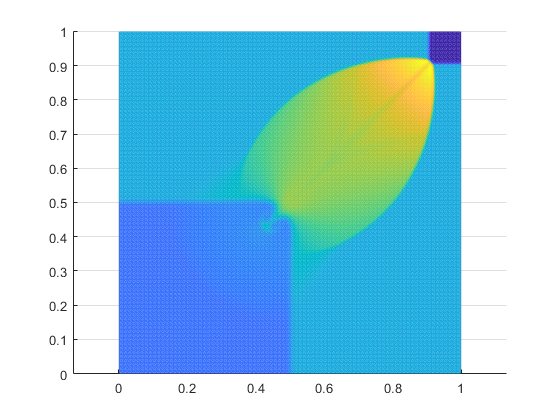
\includegraphics[width=0.45\linewidth]{fig/黎曼算例2-1.png}
        }\quad
        \subfloat{
            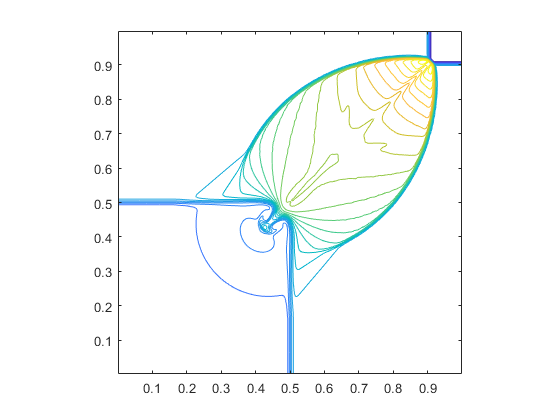
\includegraphics[width=0.45\linewidth]{fig/黎曼算例2-2.png}
        }
        \caption{WENO-JS,M=10,等高线:linspace(0.56,1.67,30)}
    \end{figure}


\end{example}


\newpage
\section{基函数函数}
对于基函数,
\cite{RN48}
\subsection{一维}
在 $[-1,1]$ 上的勒让德函数为:
\begin{equation}
    \begin{aligned}
        \varphi_{0}(\xi) & =1                                        \\
        \varphi_{1}(\xi) & =\xi                                      \\
        \varphi_{2}(\xi) & =\left(3 \xi^{2}-1\right) / 2             \\
        \varphi_{3}(\xi) & =\left(5 \xi^{3}-3 \xi\right) / 2         \\
        \varphi_{4}(\xi) & =\left(35 \xi^{4}-30 \xi^{2}+3\right) / 8
    \end{aligned}
\end{equation}
积分值为:
\begin{equation}
    \int_{-1}^{-1}\varphi_i^2\dd x=\frac{2}{2n+1},n=0,1,2,\cdots
\end{equation}

\subsection{二维}
$[-1,1]\times[-1,1]$上的勒让德函数为:
\begin{equation}
    \begin{aligned}
        \varphi_{1}(x,y) & = 1       \\
        \varphi_{2}(x,y) & = x       \\
        \varphi_{3}(x,y) & = y       \\
        \varphi_{4}(x,y) & = x^2-1/3 \\
        \varphi_{5}(x,y) & = xy      \\
        \varphi_{6}(x,y) & = y^2-1/3 \\
    \end{aligned}
\end{equation}

对于$[x_a,x_b]\times[y_a,y_b]$上的勒让德函数,只需令 $\xi=\dfrac{x - \dfrac{x_a+x_b}{2}}{\dfrac{x_b-x_a}{2}},\eta = \dfrac{y - \dfrac{y_a+y_b}{2}}{\dfrac{y_b-y_a}{2}}$
\section{数值积分}

一般采用的求积公式是机械求解求积公式中的高斯积分.高斯积分是一种非常常用的数值积分方法,具有如下优点:
\begin{itemize}
    \item 高斯积分的精度随着积分点的增加而增加,当积分点的数量足够大时,可以达到非常高的精度.
    \item 当使用的点数固定为 $n$ 个时,高斯积分具有 $2n-1$ 阶的精度,是所有机械求积公式中最高的.因此在计算复杂函数积分时,高斯积分可以显著减少计算时间和计算成本.
    \item 高斯积分公式可以非常方便地使用代码实现.
\end{itemize}
具体而言,该公式可写成:
\begin{equation}
    \int_{-1}^1 f(x)\dd x=\sum_{i=1}^{n+1}\omega_if(x_i)
\end{equation}
其中,$\omega_i$ 和 $x_i$ 分别表示高斯积分公式中第 $i$ 个点的权重和位置.对于积分区间非 $[-1,1]$ 的积分,可以使用下面的公式:
\begin{equation}
    \int_{a}^{b} f(x) \mathrm{d} x=\int_{-1}^{1} f\left(\frac{(b-a) t+b+a}{2}\right) \frac{b-a}{2} \mathrm{~d} t=\sum_i f(\frac{(b-a)x_i+b+a}{2})\frac{b-a}{2}\omega_i
\end{equation}

表 \ref{tab:Gauss-Legendre积分} 给出 $n=2,3,4,5$ 时,高斯积分的取值点和权重大小.
\begin{table}[ht]
    \centering
    \caption{Gauss-Legendre的取值点和权重大小}
    \label{tab:Gauss-Legendre积分}
    \begin{tabular}{ccc}
        \toprule
        $n$ & 取值点 $x_i$                                 & 权重 $w_i$                         \\
        \midrule
        2   & $\pm$0.57735027                              & 1.00000000                         \\
        3   & 0.00000000, $\pm$0.77459667                  & 0.88888889, 0.55555556             \\
        4   & $\pm$0.86113631, $\pm$0.33998104             & 0.34785485, 0.65214515             \\
        5   & 0.00000000, $\pm$0.53846931, $\pm$0.90617985 & 0.56888889, 0.23692689, 0.23692689 \\
        \bottomrule
    \end{tabular}
\end{table}


还有一种求积方式也称为 Gauss-Lobatto 求积,以荷兰数学家 Rehuel Lobatto 命名.它类似于高斯求积,但有以下区别:
\begin{itemize}
    \item 积分点包括积分区间的端点.
    \item 对于 $2n – 3$ 次以下的多项式,它是准确的,其中 n 是积分点的数量.
\end{itemize}
当需要使用区间断点作为积分点的时候,应当选用 Gauss-Lobatto 求积.


% https://zhuanlan.zhihu.com/p/597515168
\cite{RKDG2} reamrk 2.6


为了计算 xx 中非线性 $f$ 的积分,必须使用正确阶次的求积,以便近似误差
\begin{equation}
    \frac{1}{\Delta x_{j}^{l+1}} \int_{I_{j}} f\left(u^{h}(x, t)\right) \frac{d}{d x} v_{l}^{(j)}(x) d x
\end{equation}
为 $O\left(h^{k+1}\right)$. 我们需要使求积的误差为 $O\left(h^{2 k+2}\right)$。对于高斯积分,误差为 $O\left(h^{2n-1}\right)$,对于Gauss-Lobatto,误差为 $O\left(h^{2n-3}\right)$.

另一方面,由于我们可以在使用 Gauss-Lobatto 积分的时候,可以将 $h_{j \pm 1 / 2}$  储存起来,用于后面计算  $f\left(u^{h}\left(x_{j \pm 1 / 2}, t\right)\right)$ 从而节省计算量。所以在积分点的数量 $n$ 相同的情况下,优先使用  Gauss-Lobatto 积分。

\begin{itemize}
    \item 对于  $\mathbb{P}^{1}$  的情况, 我们使用两点高斯积分点  $x_{i-\sqrt{3} / 6}$  和  $x_{i+\sqrt{3} / 6}$ .
    \item 对于  $\mathbb{P}^{2}$  的情况, 我们使用四点 Gauss-Lobatto 积分点  $x_{i-1 / 2}, x_{i-\sqrt{5} / 10}, x_{i+\sqrt{5} / 10}$ , 和  $x_{i+1 / 2}$ .
    \item 对于  $\mathbb{P}^{3}$  的情况, 我们使用四点 Gauss 积分点  $x_{i-\sqrt{525+70 \sqrt{30}} / 70}, x_{i-\sqrt{525-70 \sqrt{30}} / 70}, x_{i+\sqrt{525-70 \sqrt{30}} / 70}$  and  $x_{i+\sqrt{525+70 \sqrt{30}} / 70}$ .
\end{itemize}

\begin{table}[ht]
    \centering
    \caption{Gauss-Lobatto的取值点和权重大小}
    \label{tab:Gauss-Lobatto积分}
    \begin{tabular}{ccc}
        \toprule
        $n$ & 取值点 $x_i$                                 & 权重 $w_i$                         \\
        \midrule
        2   & $\pm$1.00000000                              & 1.00000000                         \\
        3   & $\pm$1.00000000, 0.00000000                  & 0.33333333, 1.33333333             \\
        4   & $\pm$1.00000000, $\pm$0.44721360             & 0.16666667, 0.83333333             \\
        5   & $\pm$1.00000000, $\pm$0.65465367, 0.00000000 & 0.10000000, 0.54444444, 0.71111111 \\
        \bottomrule
    \end{tabular}
\end{table}
对于$n$不同的情况,可以从这个\cite{RN106}查到更多$x_i$,$\omega_i$的值.
\section{计算精度}
假设我们得到的近似解为 $u_h$, 准确解为 $u$.
\begin{equation}
    || u_h-u || = Ch^p + O(h^{p+1})
\end{equation}
下面介绍如何通过数值实验求出 $p$.

在两次实验中,我们使用了不同的 $h=h_1,h_2$,得到的近似解为 $u_{h_1},u_{h_2}$. 则:

\begin{equation}
    \begin{aligned}
        || u_{h_1}-u || = Ch_1^p + O(h^{p_1+1}) \\
        || u_{h_2}-u || = Ch_2^p + O(h^{p_2+1}) \\
    \end{aligned}
\end{equation}
做比得到:
\begin{equation}
    \frac{|| u_{h_1}-u ||}{|| u_{h_2}-u ||} = \left(\frac{h_1}{h_2}\right)^p
\end{equation}
于是
\begin{equation}
    p = \frac{\ln|| u_{h_1}-u ||-\ln|| u_{h_2}-u ||}{\ln(h_1)-\ln(h_2)}
\end{equation}
% 当取值为小区间中心点时:
% \begin{equation}
%     \begin{aligned}
%         L_{1}-\operatorname{norm} & =\frac{1}{n} \sum_{i=1}^{n}\left|u\left(x_{i}\right)-u h\left(x_{i}\right)\right|            \\
%         L_{2}-\text { norm }      & =\sqrt{\frac{1}{n} \sum_{i=1}^{n}\left(u\left(x_{i}\right)-u h\left(x_{i}\right)\right)^{2}} \\
%         L_{\infty}-\text { norm } & =\max x_i,i=1,2,\cdots,n                                                                     \\
%     \end{aligned}
% \end{equation}

下面给出一种使用函数积分值来计算范数的方法:假设小区间的数量为 $n$,数值解为 $u_h$,准确解为 $u$.
\begin{itemize}
    \item 对于 $L_1$ 范数,我们有:
          \begin{equation}
              || u_{h}-u || = \frac{\sum_{i=1}^{n}\int_{I_i}|u_{h}-u|\dd x }{\sum_{i=1}^{n}\int_{I_i}\dd x}
          \end{equation}

    \item 对于 $L_2$ 范数,我们有:
          \begin{equation}
              || u_{h}-u || = \sqrt{\sum_{i=1}^{n}\int_{I_i}\left(u_{h}-u\right)^2\dd x}
          \end{equation}
    \item 对于 $L_\infty$ 范数,我们有:
          \begin{equation}
              || u_{h}-u || = \max_i \left\{\frac{\int_{I_i}\left(u_{h}-u\right)^2\dd x}{} \right\}
          \end{equation}
\end{itemize}


\begin{equation}
    \begin{aligned}
        L_{1}-\operatorname{norm} & =\sum_{i=1}^{n}\left|u\left(x_{i}\right)-u h\left(x_{i}\right)\right|            \\
        L_{2}-\text { norm }      & =\sqrt{\sum_{i=1}^{n}\left(u\left(x_{i}\right)-u h\left(x_{i}\right)\right)^{2}} \\
        L_{\infty}-\text { norm } & =\max x_i,i=1,2,\cdots,n                                                         \\
    \end{aligned}
\end{equation}
\section{常用中英文对照表}
\begin{itemize}
    \item Analytical Solution : 解析解
    \item monotone: 单调
    \item consistency:一致性
    \item Shock Wave:激波
    \item Contact Wave:接触间断
    \item Rarefaction Wave:稀疏波
\end{itemize}
\section{常用期刊名缩写}
\begin{itemize}
    \item J. Comput. Phys. : Journal of Computational Physics
\end{itemize}
\section{常用缩写对照表}
\begin{itemize}
    \item CFL:Courant–Friedrichs–Lewy
    \item CFD:Computational Fluid Dynamics
    \item DG:discontinuous Galerkin
    \item DOF:Degree of Freedom
    \item ENO:essentially non-oscillatory scheme
    \item SSP:strong stability perserving
    \item TVD:total variation diminishing
    \item TVDM:total variation diminishing in the means
    \item HLLC:Harten–Lax–van Leer contact
    \item RK:Runge-Kutta
    \item FV:finite volume
    \item FD:finite difference
    \item JCP:Journal of Computational Physics
    \item PPM:piecewise parabolic method
    \item WENO:weighted essentially non-oscillatory schemes
\end{itemize}
\bibliographystyle{plain}
\bibliography{ref.bib}
\end{document}